\renewcommand{\prevlecture}{3 }
\renewcommand{\thislecture}{4 }
\renewcommand{\nextlecture}{5 }

%
% Cover page
%

\title[PHYS 201 / Lecture \thislecture]
{
  PHYS 201 / Lecture \thislecture\\
  {\it Conductors; Capacitance; Dielectrics; Dipoles; Polarization}\\
}

\author[C.Andreopoulos] {
  Professor Costas Andreopoulos\inst{1,2}, {\it FHEA}
}
\institute[Liverpool/STFC-RAL] {
   \inst{1} University of Liverpool, Department of Physics\\
   \vspace{0.1cm}
   \inst{2} U.K. Research \& Innovation (UKRI), Science \& Technology Facilities Council,\\
            Rutherford Appleton Laboratory, Particle Physics Department\\
   \vspace{0.5cm}
   {\it {\color{magenta} Lectures delivered at the University of Liverpool, 2020-21}}\\
   \vspace{0.2cm}
}
\date{\today}

\titlegraphic{
  
\includegraphics[height=25px]{./images/logo/liverpool.png}
  \hspace{3px}
  
\includegraphics[height=30px]{./images/logo/ral.png}
}


\begin{frame}[plain]
  \titlepage
\end{frame}

% ------------------------------------------------------------------------------
% ------------------------------------------------------------------------------

%
% Revision of previous lecture
%

\renewcommand{\lecturesummarytitle}{Revision }

\renewcommand{\summarizedlecture}{3 }

%
%
%

\begin{frame}{Lecture \summarizedlecture - \lecturesummarytitle}

\begin{itemize}
\item {\bf To bring together a collection of charges I need to do work}
      (for example, In case of two like-sign charges I need to exert a force against the action of the field)
      \begin{equation*}
        W = \int \vec{F} \cdot d\vec{\ell}
      \end{equation*}
\item The work done can be positive or negative.
\item The work done is {\bf path-independent}
  \begin{itemize}
     \item I do the same work regardless of the path followed to bring the charges in their positions.
     \item We say that the electric force is {\bf conservative}.
  \end{itemize}
\item The work done is converted to {\bf electric potential energy}
\item We calculated the  potential energy for systems of 2, 3 and N charges as well as continuous distributions of charge.

\end{itemize}

\end{frame}

%
%
%

\begin{frame}{Lecture \summarizedlecture - \lecturesummarytitle (cont'd)}

For a
\begin{itemize}
\item system of 2 charges:
 \begin{equation*}
      U = \frac{q_1 q_2}{4\pi\epsilon_0} \frac{1}{|\vec{r}_{12}|}
 \end{equation*}

\item system of 3 charges:
 \begin{equation*}
   U = \frac{q_1 q_2}{4\pi\epsilon_0} \frac{1}{|\vec{r}_{12}|} +
       \frac{q_1 q_3}{4\pi\epsilon_0} \frac{1}{|\vec{r}_{13}|} +
       \frac{q_2 q_3}{4\pi\epsilon_0} \frac{1}{|\vec{r}_{23}|}
 \end{equation*}

\item system of N charges:
 \begin{equation*}
   U = \frac{1}{2} \sum_{i,j=1;i{\ne}j}^{N} \frac{q_i q_j}{4\pi\epsilon_0|\vec{r}_{ij}|}
 \end{equation*}

\item continuous charge distribution (with density $\rho$ over a volume $\tau$):
 \begin{equation*}
    U = \frac{1}{2} \int_{\tau} d\tau \int_{\tau^{\prime}} d\tau^{\prime}
        \frac{\rho(\vec{r}) \rho(\vec{r^{\prime}})}{4\pi\epsilon_0|\vec{r} - \vec{r^{\prime}}|}
 \end{equation*}

\end{itemize}

\end{frame}

%
%
%

\begin{frame}{Lecture \summarizedlecture - \lecturesummarytitle (cont'd)}

\begin{itemize}
  \item
  The electric {\bf potential energy is stored in the electric field}:
  \begin{equation*}
     U = \frac{\epsilon_0}{2} \int_{all\;space} |\vec{E}(\vec{r})|^2  d\tau
  \end{equation*}

  \item
  {\bf Relationship between force and potential energy}:\\
  \begin{equation*}
     U = \int \vec{F} \cdot d\vec{\ell}
  \end{equation*}
  \begin{equation*}
     \vec{F} = -\vec{\nabla}U
  \end{equation*}

  \item
  {\bf Electric potential (V)}: A scalar field
      \begin{itemize}
          \item It is the amount of work required to bring a charge Q at position $\vec{r}$, divided by the charge Q.
          \item SI units: Volts (V)
            \begin{itemize}
               \item Derived unit: One Joule per Coulomb
            \end{itemize}
      \end{itemize}
\end{itemize}

\end{frame}

%
%
%

\begin{frame}{Lecture \summarizedlecture - \lecturesummarytitle (cont'd)}

\begin{itemize}
  \item We also studied the {\bf circuital law for Electrostatics}
     \begin{itemize}
        \item Our second set of Maxwell's equations.
     \end{itemize}
  \vspace{0.2cm}
  \item Maxwell's equation we know so far:
\end{itemize}

\begin{center}
 {
  \begin{table}[H]
    \begin{tabular}{|l|c|c|}
      \hline
          & {\it Integral form} & {\it Differential form} \\
      \hline
      {\bf Gauss's law} &
        $\oint \vec{E} \cdot d\vec{S} = Q_{enclosed} / \epsilon_0$ &
        $\vec{\nabla} \cdot \vec{E} = \rho / \epsilon_0$ \\

      {\bf Circuital law} &
        $\oint \vec{E} \cdot d\vec{\ell} = 0$ &
        $\vec{\nabla} \times \vec{E} = 0$ \\
      \hline
    \end{tabular}
  \end{table}
 }
\end{center}

\begin{itemize}
  \item Because (in Electrostatics) the electric field has no rotation
        it can be expressed as the gradient of a scalar function (the electric potential):
        \begin{equation*}
           \vec{E} = - \vec{\nabla} V
        \end{equation*}
\end{itemize}


\end{frame}

%
%
%

\begin{frame}{Lecture \summarizedlecture - \lecturesummarytitle (cont'd)}

\begin{itemize}

  \item Need both the divergence and the curl of $\vec{E}$ (both Gauss' and circuital laws)
        to determine all three components of $\vec{E}$.
    \begin{itemize}
    {
      \item Gauss' and circuital laws provide a coupled system of 1$^{st}$ order p.d.e's.
    }
    \end{itemize}

  \item I can combine the Gauss' and circuital laws into a single 2$^{nd}$ order p.d.e for the
        electric potential V: {\bf Poisson equation}
        \begin{equation*}
           \vec{\nabla}^{2} V = - \frac{\rho}{\epsilon_0}
        \end{equation*}

  \item Away from sources ($\rho$=0) Poisson's equation becomes $\vec{\nabla}^{2} V = 0$
        which is known as the {\bf Laplace equation}.

  \item Using the Poisson (or Laplace) equations one can determine V (and, thus, $\vec{E}$)
        only using the appropriate {\bf boundary conditions}.

  \item {\bf A uniqueness theorem} is a proof that a given set of boundary conditions is sufficient.

\end{itemize}

\end{frame}


%
% Plan for this lecture
%

\begin{frame}{Plan for Lecture \thislecture}

\begin{itemize}
  \item So far we studied electrostatics in the {\em vacuum}.
  \item In this lecture we will discuss {\bf what happens when materials are placed within an electric field}.

  \item With regards to their electrical properties, there are 2 main types of materials
   \begin{itemize}
     \item materials that conduct electricity: {\bf conductors}
     \item materials that do not conduct electricity: {\bf insulators (dielectrics)}
   \end{itemize}

   \item We will start by discussing what happens when we place a conductor in an electrostatic field

   \item We will discuss the concept of capacitance, and
         study in more detail a simple capacitor: Parallel plate capacitor.

   \item Then, we also see what happens when we place a dielectric inside an electrostatic field
         and we will discuss electrical dipoles and the concept of polarisation.
\end{itemize}
\end{frame}

% ------------------------------------------------------------------------------
% ------------------------------------------------------------------------------

%
%
%

\begin{frame}{Conductors}

\begin{columns}
  \begin{column}{0.70\textwidth}
    A {\bf {\em conductor}} is an object or type of material
    which {\bf contains electric charges that are relatively free to move} through that object or material.\\
  \end{column}
  \begin{column}{0.30\textwidth}
     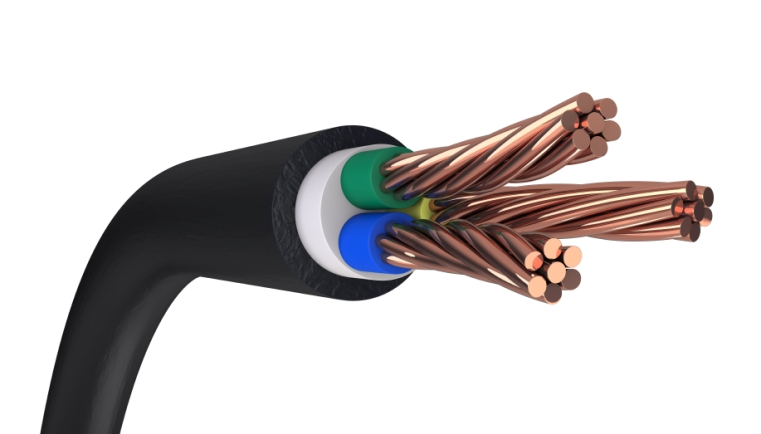
\includegraphics[width=0.95\textwidth]{./images/photos/power_cable_01.jpg}\\
  \end{column}
\end{columns}

\vspace{0.3cm}

Free electric charges:
\begin{itemize}
  \item In most case, these are {\bf electrons} (e.g. in metals).
  \item But in some cases the positive charges may also be able to move (e.g. in electrolytes such as as salt water).
\end{itemize}

\vspace{0.3cm}
A {\em \bf perfect conductor} has an {\bf unlimited supply of free charges}.

\end{frame}

%
%
%

\begin{frame}{Supply of free charges}

What provides that {\em unlimited supply} of free charges?\\
We will examine the most typical conducting substance: {\bf Metals}.\\

\begin{center}
   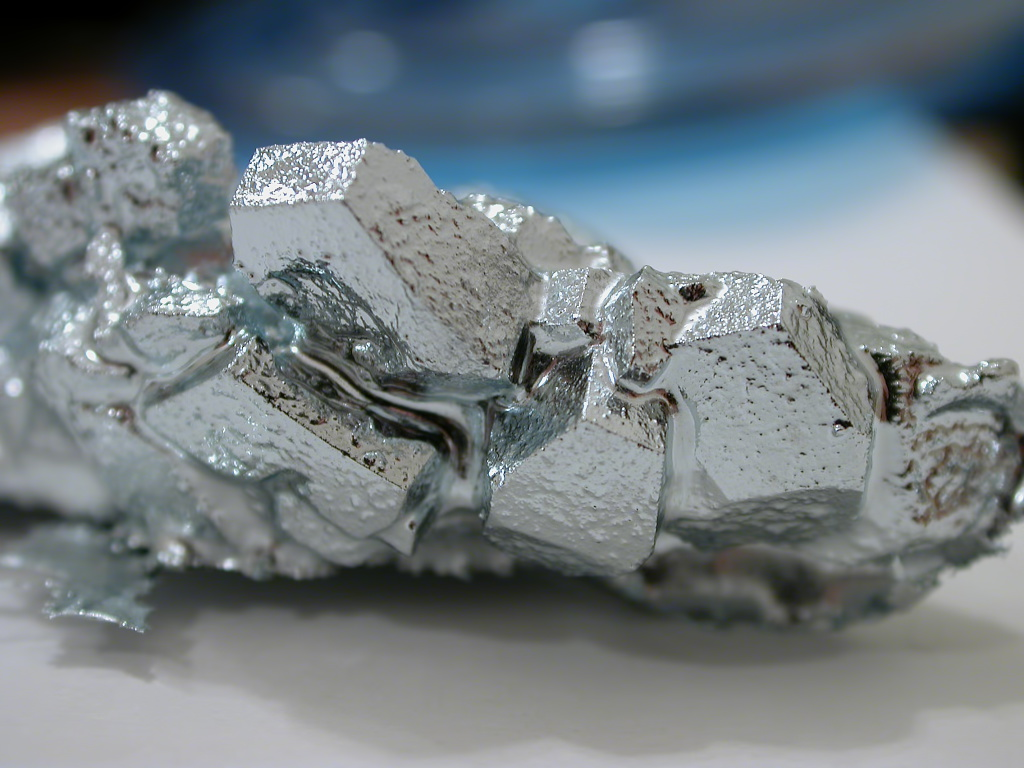
\includegraphics[width=0.70\textwidth]{./images/photos/gallium_crystals.jpg}
\end{center}

\end{frame}

%
%
%

\begin{frame}{Crystal structure of metals}

In a metallic substance, the {\bf atoms are usually closed packed and neatly arranged
in symmetrical structures we call {\em crystals}}.\\
\vspace{0.2cm}
\begin{itemize}
  \item Think how grocers pack oranges: Nature does something very similar when it organizes
        atoms in crystals.
  \item Atoms in crystals typically have 12 or 8 touching neighbours.
\end{itemize}

\begin{columns}
  \begin{column}{0.50\textwidth}
      \begin{center}
         {\bf 12 neighbours} \\
         \vspace{0.23cm}
         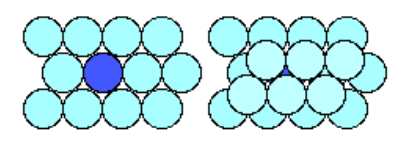
\includegraphics[width=0.80\textwidth]{./images/schematics/crystals_12_touching_neighbours.png}
      \end{center}
      {\scriptsize
        6 neighbours on each plane + 3 on each of the two neighbouring planes.\\
      }
  \end{column}
  \begin{column}{0.50\textwidth}
      \begin{center}
         {\bf 8 neighbours} (less efficient packing) \\
         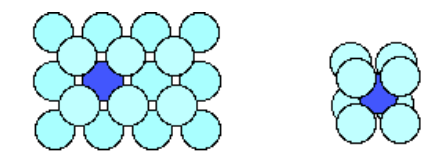
\includegraphics[width=0.80\textwidth]{./images/schematics/crystals_8_touching_neighbours.png}
      \end{center}
      {\scriptsize
        No touching neighbour on same plane, but 4 from each of the planes below and above.\\
      }
  \end{column}
\end{columns}

\end{frame}

%
%
%

\begin{frame}{Supply of free charges}

{\bf Atoms lose one or more electrons from their outer shells and these electrons are free to move}.
In the case of metals the positive charges are packed together and can not move.\\

\begin{columns}
  \begin{column}{0.50\textwidth}
      \begin{center}
        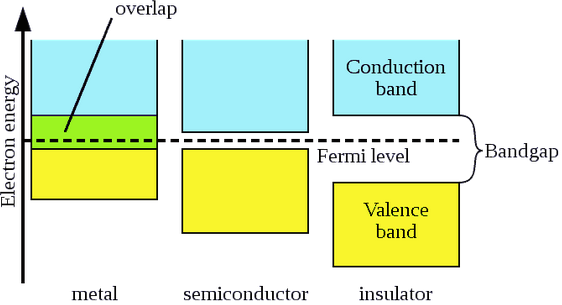
\includegraphics[width=0.98\textwidth]{./images/schematics/conduction_band.png}\\
      \end{center}
  \end{column}
  \begin{column}{0.50\textwidth}
    \begin{itemize}
    {\scriptsize
      \item Energy levels quantized.
      \item Closely spaced levels: Energy "bands".
      \item Nature seeks to minimize the total energy but not all electrons in the lowest state (Pauli exclusion principle).
      \item Levels up to the Fermi level are filled.
      \item Metals have many energy levels close to the Fermi level: Electrons can jump between states.\\
    }
    \end{itemize}
  \end{column}
\end{columns}

\vspace{0.3cm}

A {\em \bf perfect conductor} has an {\bf unlimited supply of free charges}.
\begin{itemize}
  \item There are no perfect conductors, but many substances come close!
  \item For example, in copper, the free charge density is 1.8 $\times$ 10$^{10}$ C/m$^3$.
\end{itemize}

\end{frame}

%
%
%

\begin{frame}{Placing a conductor within an electric field}

{\bf What happens if we place a conductor} (e.g. a chunk of metal)
{\bf within an external electric field?}\\
\vspace{0.3cm}

\begin{itemize}
  \item The electric field vanishes everywhere inside a conductor.
  \item The potential in constant inside a conductor.
  \item Charge accumulates in the surface.
  \item The electric field on the surface of a conductor has no tangential component.
\end{itemize}

\vspace{0.2cm}
How do these effects come about?

\end{frame}


%
%
%

\begin{frame}{The effect of the external electric field}

Assume that our conductor is uncharged, so it is neutral (*).
Of course, it is made up from positive and negative charges.
Within an external field:
\begin{itemize}
{\small
 \item The free negative charges will move opposite to the field.
 \item The positive charges feel a force but are pinned and can not move.
}
\end{itemize}

\begin{columns}
  \begin{column}{0.50\textwidth}
      \begin{center}
        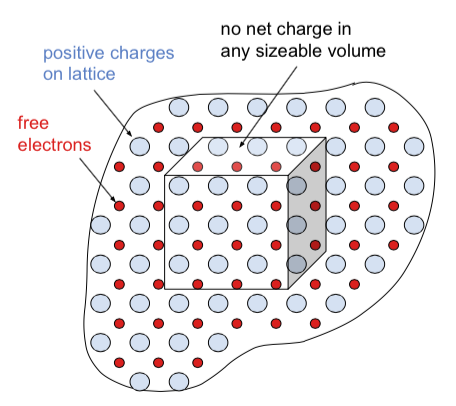
\includegraphics[width=0.75\textwidth]{./images/schematics/metal_in_electric_field_1.png}\\
      \end{center}
  \end{column}
  \begin{column}{0.50\textwidth}
      \begin{center}
        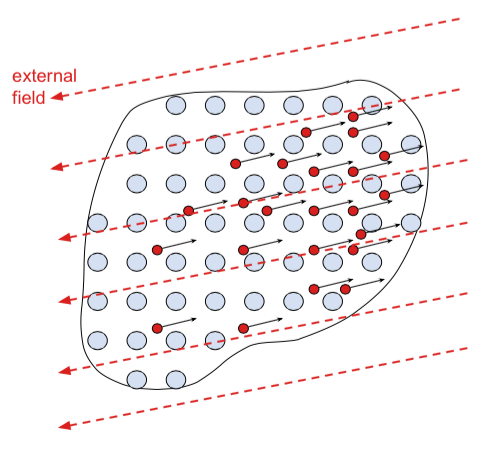
\includegraphics[width=0.80\textwidth]{./images/schematics/metal_in_electric_field_2.png}\\
      \end{center}
  \end{column}
\end{columns}

\noindent\rule{2cm}{0.4pt}\\
{\scriptsize
 (*) It is neutral on average: i.e. in {\em macroscopic} volumes that contain few $\times$ $\sim$100 atoms.
 Obviously much smaller volumes can have net charge:
 For example, a volume that includes only an atomic nucleus will be positively charged.\\
}

\end{frame}

%
%
%

\begin{frame}{The electric field inside a conductor}

The motion of charges creates a {\bf macroscopic accumulation of charge}:
\begin{itemize}
{\small
  \item An excess of negative charge on the side opposite to the
        direction of $\vec{E}$.
  \item A deficit of negative charge (i.e. an excess of positive charge)
        on the side pointed to by $\vec{E}$.
}
\end{itemize}

\begin{columns}
  \begin{column}{0.45\textwidth}
      \begin{center}
        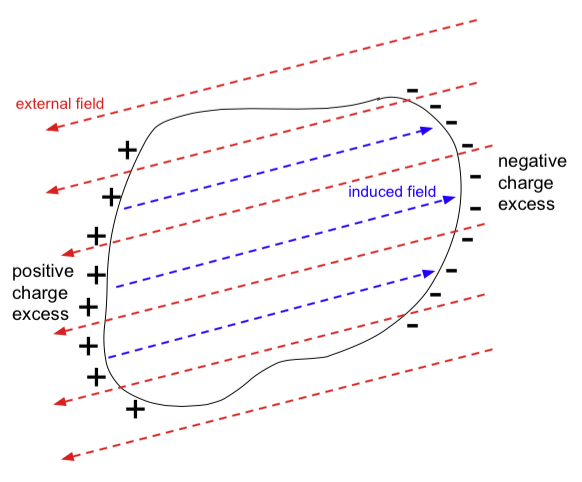
\includegraphics[width=0.98\textwidth]{./images/schematics/metal_in_electric_field_3.png}\\
      \end{center}
  \end{column}
  \begin{column}{0.55\textwidth}
  \begin{itemize}
   {\small
   \item {\bf The induced charges create an electric field of their own}.
   \item The electric field within the conductor is the vector sum of the the external and induced fields.
   \item The induced electric field {\bf opposes the external field}.
   }
  \end{itemize}
  \end{column}
\end{columns}

\vspace{0.2cm}
Eventually {\bf the electric field vanishes {\em everywhere} inside the conductor.}\\

\end{frame}

%
%
%

\begin{frame}{The electric potential inside a conductor}

Recall that the electric field $\vec{E}$ and electric potential V are related as follows:
\begin{equation*}
  \vec{E} =
     - \vec{\nabla} V =
     - \Big(
          \frac{\partial V}{\partial x},
          \frac{\partial V}{\partial y},
          \frac{\partial V}{\partial z}
       \Big)
\end{equation*}

\vspace{0.3cm}

The electric field vanishes everywhere inside a conductor.\\
\vspace{0.3cm}

Therefore, {\textbf{the potential in constant inside a conductor.}}\\
\vspace{0.2cm}
We say that the conductor is an {\bf equipotential}.\\

\end{frame}

%
%
%

\begin{frame}{Induced charge inside a conductor}

As we have seen, charges are free to move. Where to?\\
\vspace{0.3cm}
{\bf The surface} is the only place where induced charges could be!
\begin{itemize}
  \item It follows from Gauss's law:
    \begin{equation*}
       \vec{\nabla} \cdot \vec{E} = {\rho}/\epsilon_0
    \end{equation*}
  \item If $|\vec{E}|=0$ inside a conductor, then $\rho(r)$=0 too.
  \item The induced charges can not live in the volume of the conductor, so they have to be on its surface.
\end{itemize}


\end{frame}


%
%
%

\begin{frame}{Field on the surface of the conductor}

\begin{columns}
  \begin{column}{0.40\textwidth}
      \begin{center}
        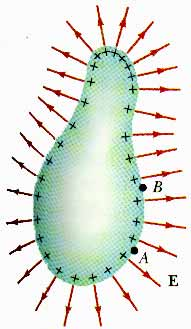
\includegraphics[width=0.85\textwidth]{./images/schematics/conductor_irregular_shape_surface_field.jpg}\\
      \end{center}
  \end{column}
  \begin{column}{0.60\textwidth}
    For the same reasons that the electric field is cancelled off within the conductor,
    {\bf it is perpendicular to the surface just outside the conductor}.\\
    \vspace{0.3cm}
    If there was a tangential component on the surface,
    charge would move so as to cancel off that component!\\
  \end{column}
\end{columns}

\end{frame}


%
%
%

\begin{frame}{Field on the surface of the conductor}

To be convinced, consider a charge Q moving on the surface of the conductor:\\
\vspace{0.3cm}
\begin{itemize}
  \item The electric field exerts a force upon Q.
  \item The surface of the conductor is at the same potential V.
  \item Therefore, as long as Q stays on the surface, the electric force acting on Q does no work.
\end{itemize}

\vspace{0.3cm}

Recall that $W = \int \vec{F} \cdot d\vec{\ell}$.\\

\vspace{0.3cm}

If the electric force does no work, it is because {\bf it has no tangential
component on the surface of the conductor}, i.e. it is always perpendicular to the surface.

\end{frame}


%
%
%

\begin{frame}{Field on the surface of the conductor}

Another easy way to see that the electric field just outside the surface
of a conductor has no tangential component
is by a straightforward application of the circuital law.\\

\vspace{0.3cm}

\begin{columns}
  \begin{column}{0.30\textwidth}
   \begin{center}
     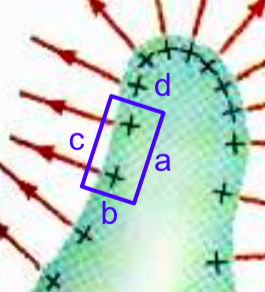
\includegraphics[width=0.99\textwidth]{./images/schematics/conductor_no_tangential_component_circuital_law.png}\\
   \end{center}
  \end{column}
  \begin{column}{0.70\textwidth}
     We know that the circulation of the electric field $\vec{E}$ along a closed trajectory is 0:
     \begin{equation*}
       \oint \vec{E} \cdot d\vec{\ell} = 0.
     \end{equation*}
     Applying the circuital law for the closed trajectory shown on the left, we have:
     \begin{equation*}
       \oint \vec{E} \cdot d\vec{\ell} =
        \int_{a} \vec{E} \cdot d\vec{\ell} + \int_{b} \vec{E} \cdot d\vec{\ell}
        + \int_{c} \vec{E} \cdot d\vec{\ell} + \int_{d} \vec{E} \cdot d\vec{\ell} = 0.
     \end{equation*}
  \end{column}
\end{columns}

\end{frame}

%
%
%

\begin{frame}{Field on the surface of the conductor}

\begin{columns}
  \begin{column}{0.30\textwidth}
   \begin{center}
     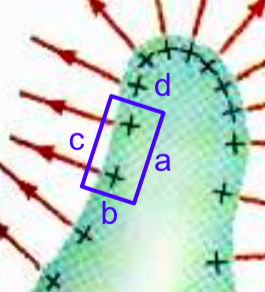
\includegraphics[width=0.99\textwidth]{./images/schematics/conductor_no_tangential_component_circuital_law.png}\\
   \end{center}
  \end{column}
  \begin{column}{0.70\textwidth}
     \begin{itemize}
       \item $\vec{E}=0$ in the conductor so the segment `a' does not contribute
             to the integral ($\int_{a} \vec{E} \cdot d\vec{\ell} = 0$).
       \item The segments exiting the conductor (`b' and `d') can be made infinitesimally small,
             so they do not contribute to the integral either\\
             ($\int_{b} \vec{E} \cdot d\vec{\ell} = \int_{d} \vec{E} \cdot d\vec{\ell} = 0$).
       \item Therefore $\oint \vec{E} \cdot d\vec{\ell} = 0$ implies that $\int_{c} \vec{E} \cdot d\vec{\ell} = 0$
     \end{itemize}
  \end{column}
\end{columns}

\begin{itemize}
  \item The segment `c' can be anywhere just outside the surface of the conductor and, since the segments `b' and `d' are
        infinitesimally small, `c' is parallel to the surface of the conductor.
  \item Therefore, the only way that $\int_{c} \vec{E} \cdot d\vec{\ell}$ to be always 0 is for $\vec{E}$ to be
        always perpendicular to the surface of the conductor.
\end{itemize}

\end{frame}



%
%
%

\begin{frame}{Distribution of charge over the surface of a conductor}

{\bf In general}, the induced charges are {\bf not uniformly distributed}.\\
\vspace{0.4cm}

Consider two conducting spheres with different radii.\\
\vspace{0.2cm}

\begin{columns}
  \begin{column}{0.33\textwidth}
  {\small
      \begin{center}
        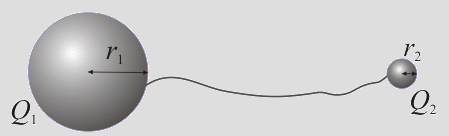
\includegraphics[width=0.90\textwidth]{./images/schematics/two_electrically_connected_spheres.png}
      \end{center}
  }
  \end{column}
  \begin{column}{0.67\textwidth}
  {\small
    The sphere with radius $r_1$ has charge $Q_1$, while the sphere with radius $r_2$ has charge $Q_2$.
    The spheres are brought into electrical contact and then separated.
  }
  \end{column}
\end{columns}

\vspace{0.3cm}

{\bf What is the charge density after separation?}\\

\vspace{0.3cm}

After the separation the two spheres have charge $Q_1^{\prime}$, $Q_2^{\prime}$
and they are at the same potential V:
\begin{equation*}
   V = \frac{Q_1^{\prime}}{4\pi \epsilon_0 r_1} = \frac{Q_2^{\prime}}{4\pi \epsilon_0 r_2}
\end{equation*}

\end{frame}

%
%
%

\begin{frame}{Distribution of charge over the surface of a conductor}

Therefore the surface charge densities are:
\begin{equation*}
   \sigma_1^{\prime} =
       \frac{Q_1^{\prime}}{4\pi r_1^2} =
       \frac{4 \pi \epsilon_0 r_1 V}{4\pi r_1^2} =
       \frac{\epsilon_0 V}{r_1}
    \;\;\;\; and \;\;\;\;
   \sigma_2^{\prime} = \frac{\epsilon_0 V}{r_2}
\end{equation*}

\vspace{0.2cm}

Thus {\bf $\sigma^{\prime} \propto \frac{1}{r}$}.\\
\vspace{0.2cm}

This is a more general conclusion.\\
\vspace{0.2cm}

\begin{columns}
  \begin{column}{0.50\textwidth}
      \begin{center}
        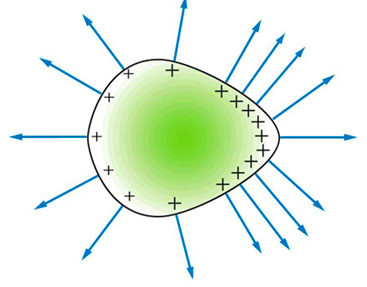
\includegraphics[width=0.90\textwidth]{./images/schematics/distribution_of_charge_over_surface_of_conductor.png}\\
      \end{center}
  \end{column}
  \begin{column}{0.40\textwidth}
    {\bf The surface charge density is smaller in the areas where curvature is smaller.}\\
  \end{column}
\end{columns}

\end{frame}

%
%
%

\begin{frame}{Summary: Placing a conductor within an electric field}

\begin{itemize}
  \item The electric field vanishes everywhere inside a conductor.
  \item The potential in constant inside a conductor.
  \item Charge accumulates in the surface.
  \item The electric field on the surface of a conductor has no tangential component.
\end{itemize}


\end{frame}


%
% Quiz
%


{
\problemslide

\begin{frame}{Quiz}

\begin{blockexmplque}{Question}
 An uncharged spherical conductor entered at the origin has a cavity with an
 arbitrary shape carved  out of it. Somewhere within the cavity is a charge q.
 What is the field outside the sphere?\\
 \begin{center}
     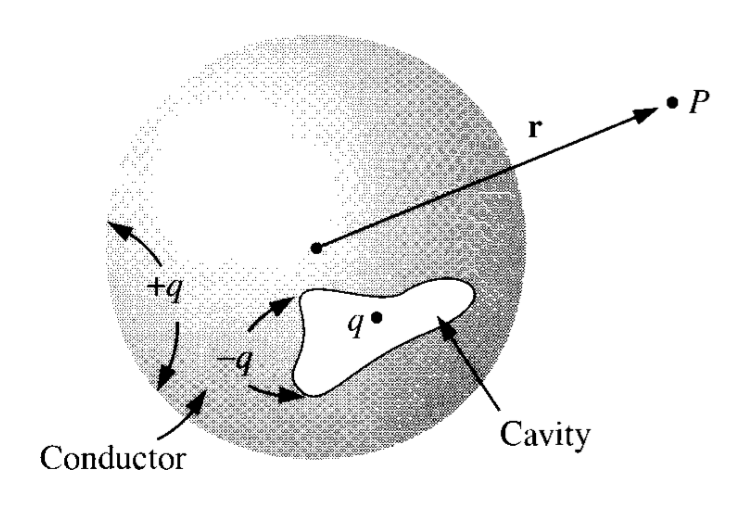
\includegraphics[width=0.47\textwidth]{./images/problems/lect3_conductor_cavity.png}
 \end{center}
\end{blockexmplque}

\vspace{0.1cm}

{\small
\it Will discuss in the lecture. For a detailed written answer see Griffiths.
}

\end{frame}


} % Worked example



%
%
%

\begin{frame}{Capacitance}

{\bf Capacitance denotes the ability of a body to store electric charge.}\\
\vspace{0.4cm}
A system that has capacitance is called a {\bf capacitor}.\\
\vspace{0.2cm}
As we shall see, capacitors store energy (in their electric field).\\
\begin{columns}
  \begin{column}{0.50\textwidth}
   \begin{center}
     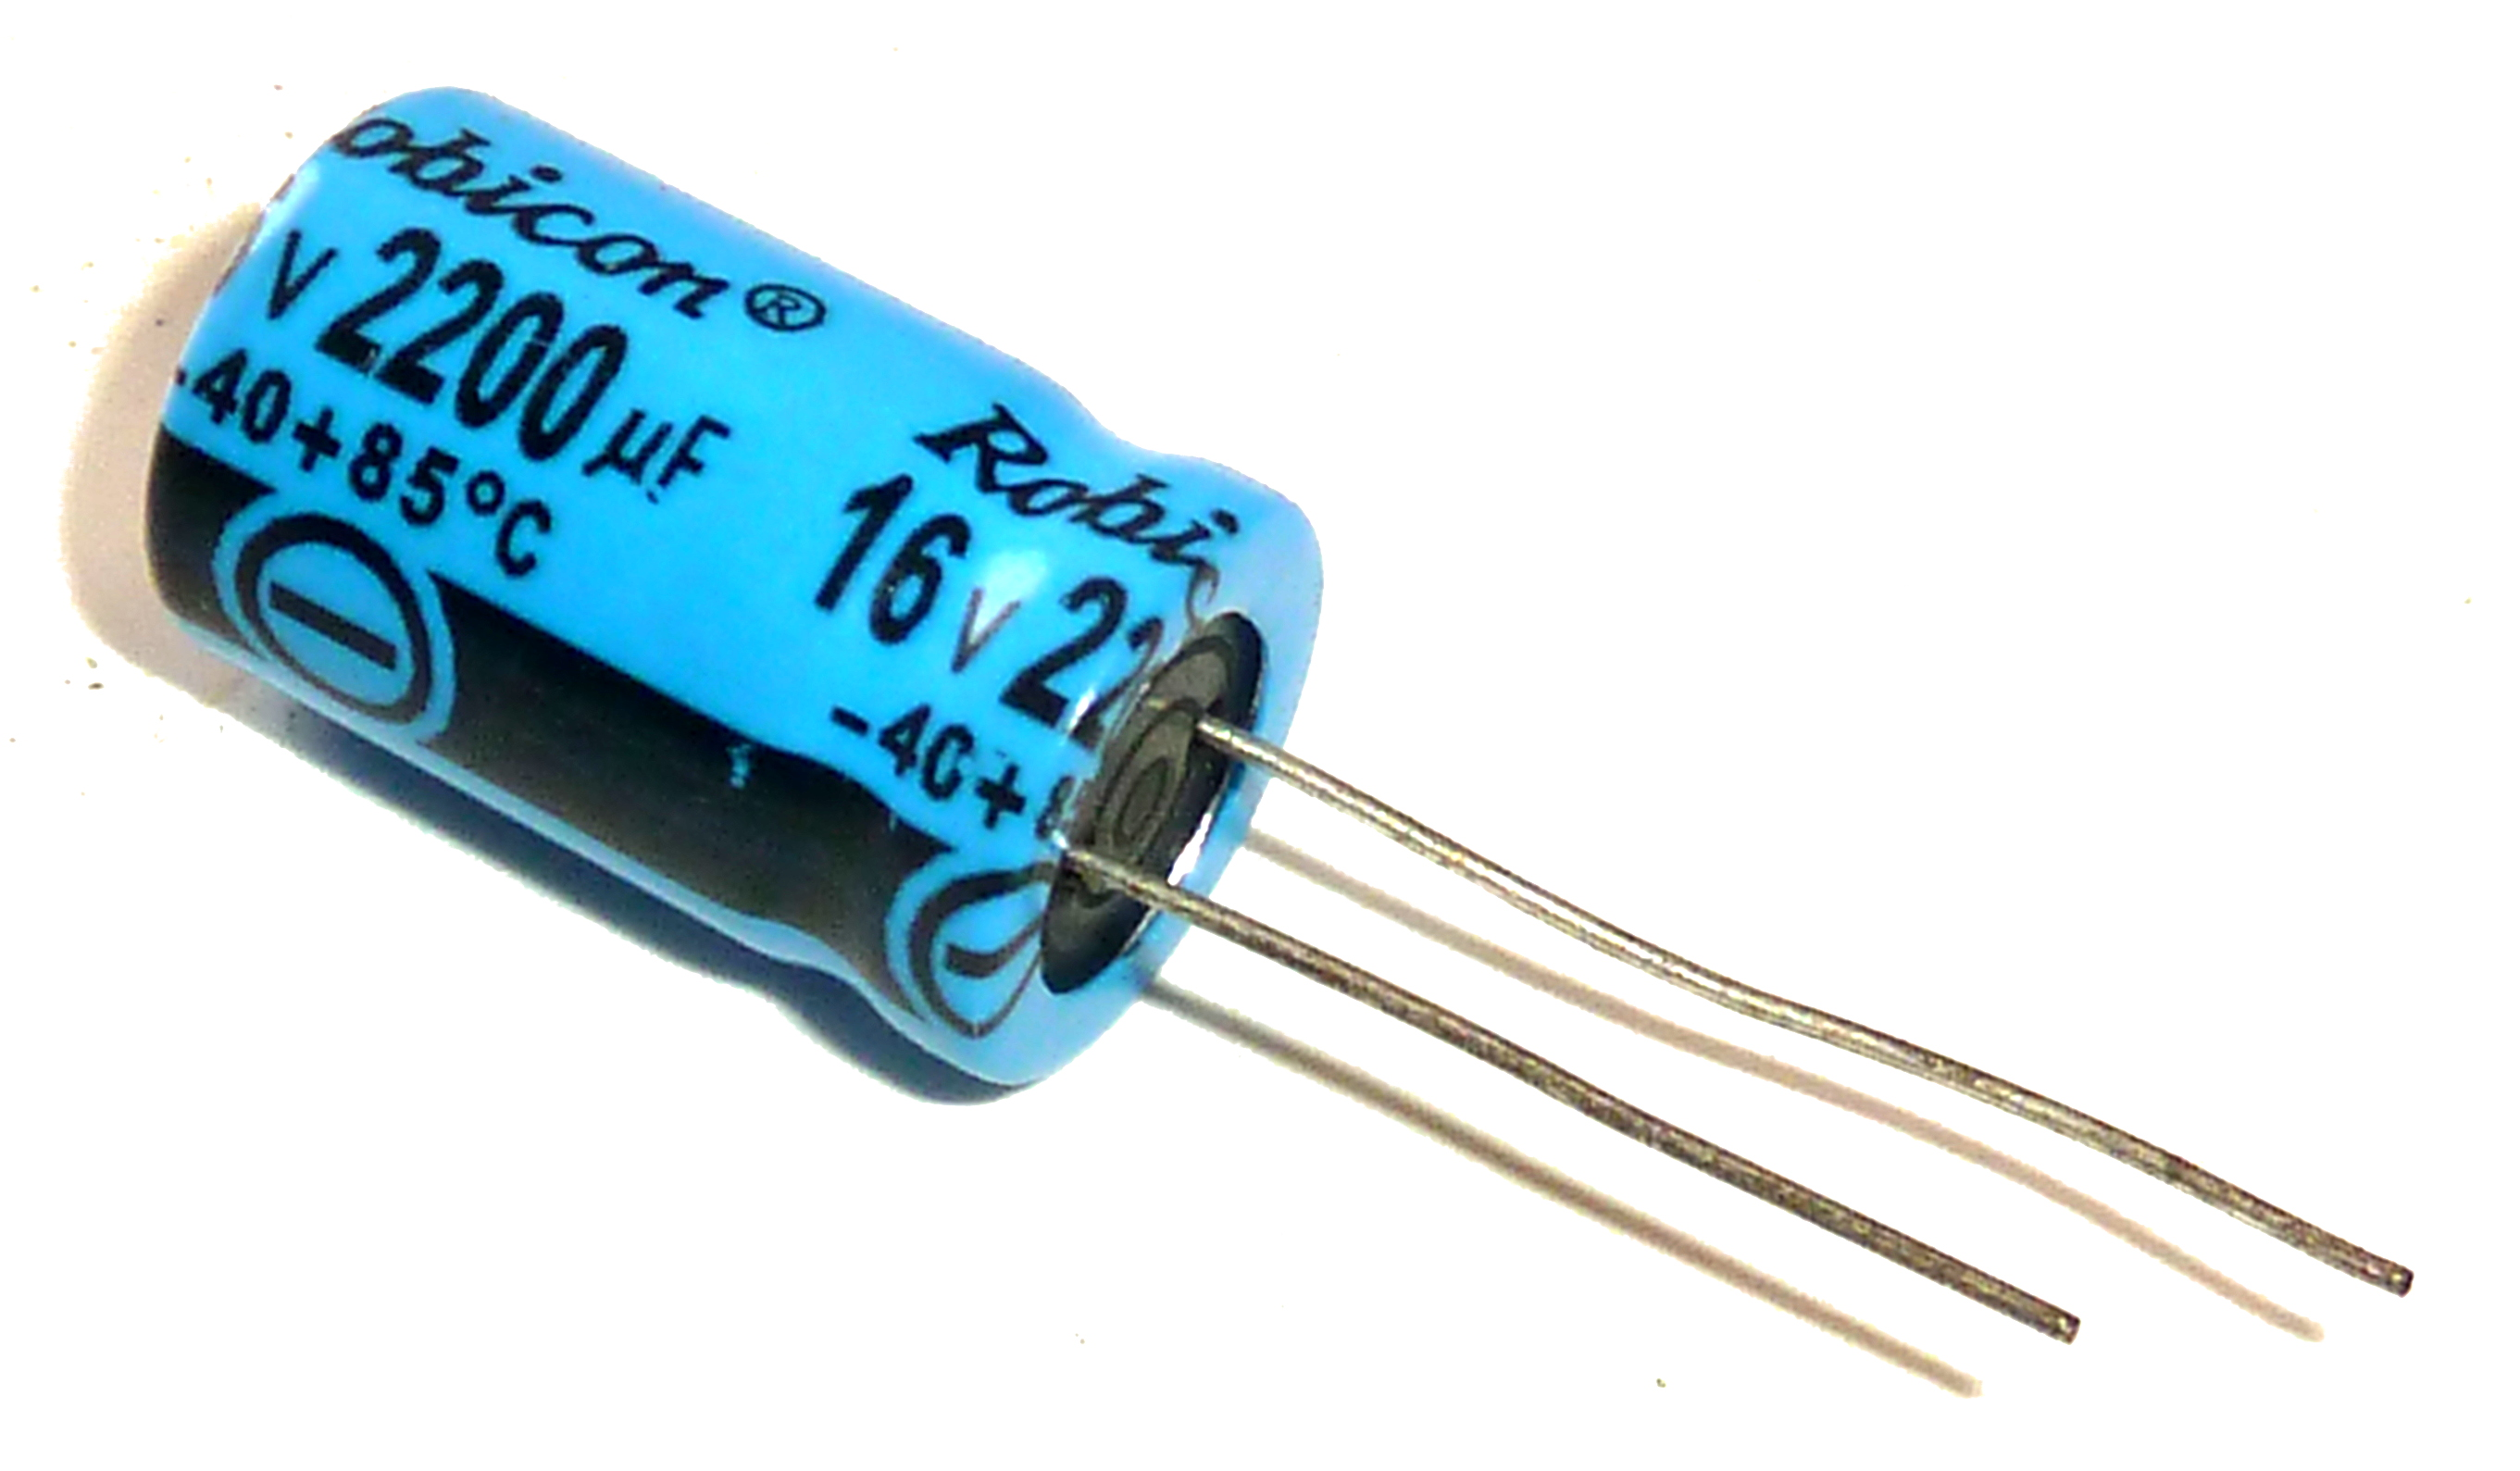
\includegraphics[width=0.95\textwidth]{./images/photos/capacitor_1.jpg}\\
   \end{center}
  \end{column}
  \begin{column}{0.50\textwidth}
   \begin{center}
     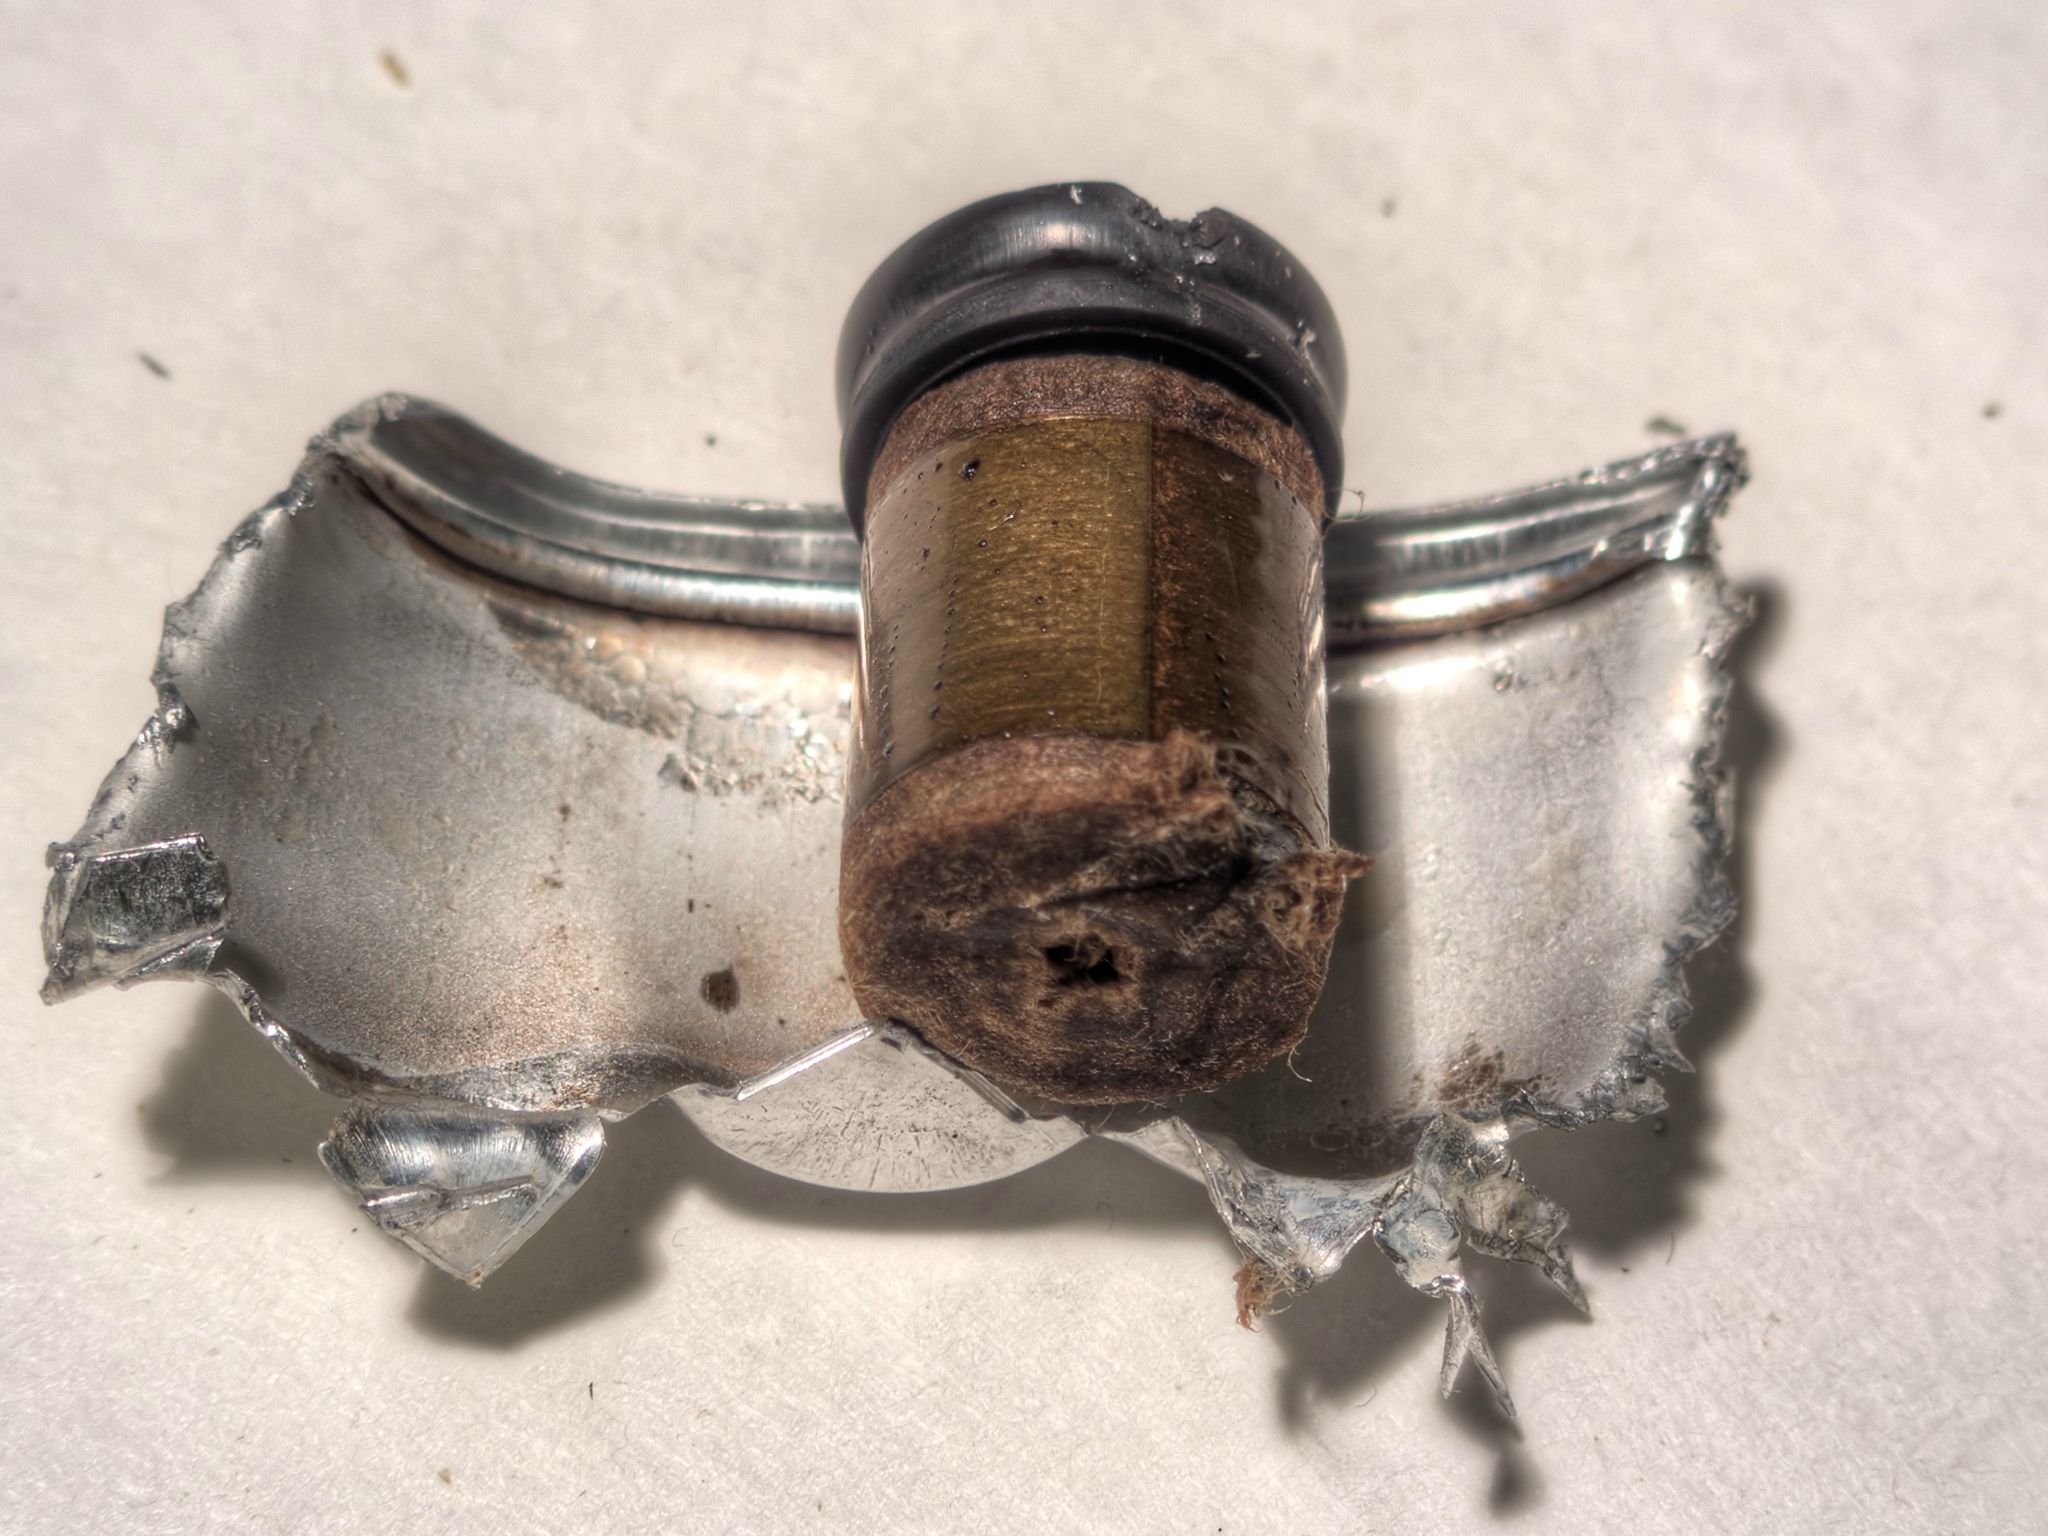
\includegraphics[width=0.95\textwidth]{./images/photos/capacitor_interior_1.jpg}\\
   \end{center}
  \end{column}
\end{columns}

\end{frame}


%
%
%

\begin{frame}{Capacitance of an isolated conductor}

At first, let's consider an {\bf isolated conductor} with {\bf net charge} Q in it.
\begin{itemize}
  \item If Q is positive that means that we took away electrons or,
  \item if Q is negative that means that we gave it an excess of electrons.
\end{itemize}

\vspace{0.3cm}

The charge Q distributes itself in the conductor.
\begin{itemize}
  \item That charge distribution is expressed with the charge density $\rho$.
  \item We don't know what that charge density is:
        The charge will not be uniformly distributed, unless the conductor is a uniform sphere.
\end{itemize}

\vspace{0.3cm}

The one thing we do know for sure is that the integral of $\rho$ over the volume of the conductor is Q
\begin{equation*}
  Q = \int_{\tau} \rho(\vec{r})d\tau
\end{equation*}

\end{frame}

%
%
%

\begin{frame}{Capacitance of isolated conductor}

As we saw earlier, the electric field is 0 within the conductor, therefore
the conductor is an {\bf equipotential}. The potential is:
\begin{equation*}
  V = \frac{1}{4\pi\epsilon_0} \int_{\tau} \frac{\rho(\vec{r})}{r} d\tau
\end{equation*}

Let's tweak the amount of charge by a factor k (e.g. let's double it (k=2)):
\begin{equation*}
  Q \rightarrow Q^{\prime} = k Q \Rightarrow
  \rho(\vec{r}) \rightarrow \rho^{\prime}(\vec{r}) = k \rho(\vec{r})
\end{equation*}

The potential changes by the same amount:
\begin{equation*}
  V \rightarrow V^{\prime} =
    \frac{1}{4\pi\epsilon_0} \int_{\tau} \frac{\rho^{\prime}(\vec{r})}{r} d\tau =
    \frac{1}{4\pi\epsilon_0} \int_{\tau} \frac{k \rho(\vec{r})}{r} d\tau =
    k \frac{1}{4\pi\epsilon_0} \int_{\tau} \frac{\rho(\vec{r})}{r} d\tau =
    k V
\end{equation*}

Therefore, {\bf the ratio Q/V remains constant}.\\
{\bf Capacitance} is the constant of proportionality (Q/V).

\end{frame}


%
%
%

\begin{frame}{Capacitance}

{\bf Capacitance} is the constant ratio Q/V.\\

\begin{itemize}
  \item In SI, capacitance has units of Coulomb/Volt (= Farad, F)\\
  \begin{itemize}
     \item So, a 1 F capacitor can store charge of 1 C at 1 V.
  \end{itemize}
\end{itemize}

The Farad is a \underline{very large unit} of capacitance.
\begin{itemize}
  \item The Earth has a capacitance of ...0.0007 F!
  \item In common electrical circuits,
        capacitors of the order of pF ($10^{-12}$F) - $\mu$F ($10^{-6}$F) are used.
\end{itemize}

\noindent\rule{2cm}{0.4pt}\\
{\scriptsize
  Consider a common AAA battery:
  \begin{itemize}
  {\small
    \item produces a nominal voltage of 1.5 V, and
    \item has a lifetime of $\sim$1 A*h = 1 C/s * 3600 s = 3600 C
  }
  \end{itemize}
  You would need a $\sim$2000 F capacitor to store
  the same amount of charge in the same potential difference!
  {\bf Impractical to use capacitors "as batteries"}.\\
  But an advantage of a capacitor is that it can discharge very very quickly,
  whereas a battery takes a long time.\\
}

\end{frame}

%
%
%

\begin{frame}{Capacitance of a system of two conductors}

Consider an {\bf isolated system of 2 conductors}.\\

\vspace{0.2cm}
If I move charge from one to another,
the two conductors become oppositely charged.
\begin{itemize}
{\small
  \item the one that loses e- becomes positively charged (+Q) and is held at potential $V_{+}$, while
  \item the one that gains e- becomes negatively charged (-Q) and is held at potential $V_{-}$
}
\end{itemize}

\vspace{0.2cm}

I can define the {\bf capacitance of the system of two conductors} as
the ratio of charge Q stored in each of the conductors over the potential difference between the two conductors:
\begin{equation*}
  C = \frac{Q}{V_{+}-V_{-}}
\end{equation*}

\end{frame}

%
%
%

\begin{frame}{Capacitance}

Capacitance is really always defined for a system of two conductors.
\begin{equation*}
  C = \frac{Q}{V_{+}-V_{-}}
\end{equation*}

What about the capacitance of the {\em single} conductor we saw earlier?\\
One can always assume that there is a second conductor at infinity held at zero potential.\\

\vspace{0.2cm}

The capacitance is an {\bf intrinsically positive quantity}.
\begin{itemize}
  \item Q is the charge of the positive conductor.
  \item $V_{+}-V_{-}$ is the positive potential difference between the positively and negatively charged conductors
     %(+ charge -> + potential; - charge -> - potential).
\end{itemize}


\end{frame}


%
%
%

\begin{frame}{Calculating the capacitance}

It is {\bf easy to calculate the capacitance for simple geometries}.\\
\vspace{0.2cm}
For example:
\begin{itemize}
  \item for a system of parallel plates, or
  \item systems with cylindrical or spherical symmetry
\end{itemize}

\begin{columns}
  \begin{column}{0.33\textwidth}
   \begin{center}
     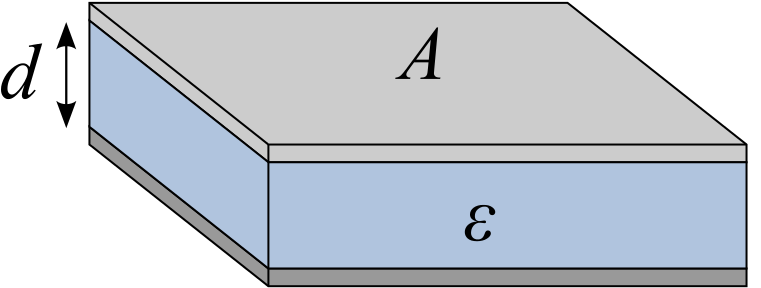
\includegraphics[width=0.75\textwidth]{./images/schematics/capacitors_parallel_plate_1.png}\\
   \end{center}
  \end{column}
  \begin{column}{0.33\textwidth}
   \begin{center}
     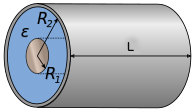
\includegraphics[width=0.75\textwidth]{./images/schematics/capacitors_cylindrical_1.png}\\
   \end{center}
  \end{column}
  \begin{column}{0.33\textwidth}
   \begin{center}
     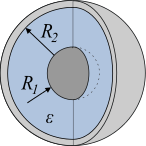
\includegraphics[width=0.75\textwidth]{./images/schematics/capacitors_spherical_1.png}\\
   \end{center}
  \end{column}
\end{columns}

\vspace{0.2cm}
In this lecture we will study the parallel plate capacitor in some detail.\\

\vspace{0.2cm}
But, first, we will discuss how we can go about calculating the capacitance in all cases.\\

\end{frame}

%
%
%

\begin{frame}{Calculating the capacitance}

For system that exhibits some spatial symmetry,
Gauss' law in integral form provides an easy way to calculate the electric field $\vec{E}$
and express it in terms of the charge Q stored in one of the conductors
(by using an appropriate Gaussian surface):
\begin{equation*}
  \oint_{S} \vec{E} \cdot d\vec{S} = \frac{Q}{\epsilon_0}
\end{equation*}

If $\vec{E}$ is known, one can calculate the potential difference V between the two conductors as:
\begin{equation*}
  V := {\Delta}V = V_{+} - V_{-} = - \int_{-}^{+} \vec{E} \cdot d\vec{\ell}
\end{equation*}

Knowing the charge Q in each conductor and
the potential difference V between the two conductors,
we calculate the capacitance C:
\begin{equation*}
  C = \frac{Q}{V}
\end{equation*}

\end{frame}


%
%
%

\begin{frame}{A simple system: Parallel plate capacitor}

We will study a simple system: The {\bf parallel plate capacitor}.\\
It consists of two planar conductors with infinitesimally small thickness.\\

\vspace{0.2cm}

\begin{columns}
  \begin{column}{0.40\textwidth}
   \begin{center}
     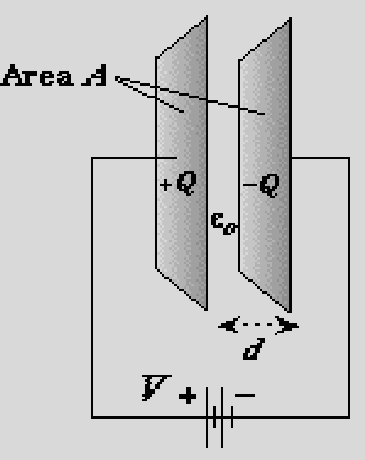
\includegraphics[width=0.94\textwidth]{./images/schematics/parallel_plate_capacitor.png}\\
   \end{center}
  \end{column}
  \begin{column}{0.60\textwidth}
  {\small
    Assume that:
    \begin{itemize}
    {\small
       \item Each plate has an area A.
       \item The two plates are at a distance d apart.
       \item The plates have a surface charge density $\sigma$ and they are oppositely charged:
         \begin{itemize}
            \item one plate has a charge $Q = \sigma A$, while
            \item the other has charge $-Q = -\sigma A$
         \end{itemize}
       \item The +Q plate is at x=0, while the -Q plate is at x=d.
       \item For now, let's consider that the two plates are separated by vacuum.
     }
     \end{itemize}
  }
  \end{column}
\end{columns}

\end{frame}

%
%
%

\begin{frame}{A simple system: Parallel plate capacitor}

We {\bf consider ideal systems} (*):
They produce symmetric field with no fringe effects (see Fig. (a)) at the edges.\\
\vspace{0.1cm}
The field produced by the parallel plate capacitor is shown in Fig. (b).\\

\begin{center}
   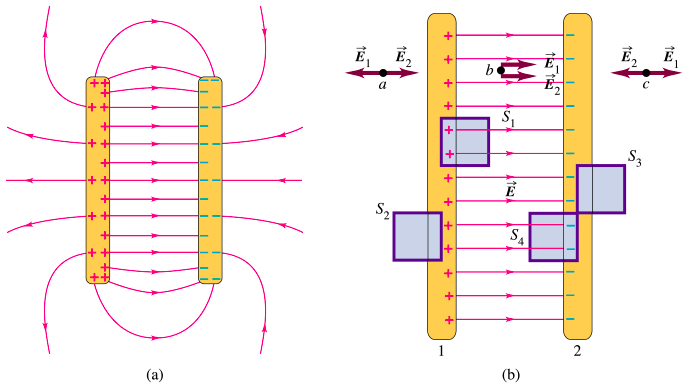
\includegraphics[width=0.70\textwidth]{./images/schematics/parallel_plate_capacitor_field.png}\\
\end{center}

\noindent\rule{2cm}{0.4pt}\\
{\scriptsize
 (*) Our main emphasis is on the concepts.
}

\end{frame}

%
%
%

\begin{frame}{Capacitance of parallel plate capacitor}

Consider the Gaussian surface shown below (dashed lines) around the plate with positive charge Q = $\sigma$A.\\
\vspace{0.1cm}

Gauss's law gives us the electric field $\vec{E}$ between the two plates.\\
\vspace{0.2cm}

\begin{columns}
  \begin{column}{0.30\textwidth}
   \begin{center}
     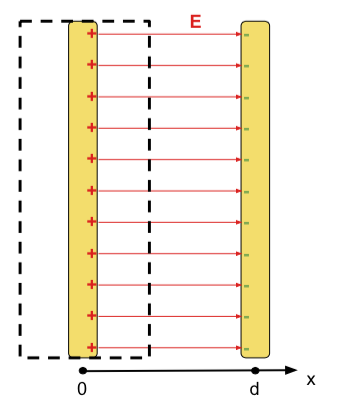
\includegraphics[width=0.99\textwidth]{./images/schematics/parallel_plate_capacitor_gaussian_surface.png}\\
   \end{center}
  \end{column}
  \begin{column}{0.70\textwidth}
     \begin{equation*}
       \oint_{A} \vec{E} \cdot d\vec{S} = \frac{Q_{enc}}{\epsilon_0} \Rightarrow
       \oint_{A} \big( E \hat{x} \big) \cdot \big( dS \hat{x} \big) = \frac{\sigma A}{\epsilon_0} \Rightarrow
     \end{equation*}

     \begin{equation*}
       E (\hat{x} \cdot \hat{x}) \oint_{A} dS = \frac{\sigma A}{\epsilon_0} \xRightarrow{\hat{x}\cdot\hat{x}=1}
       E A = \frac{\sigma A}{\epsilon_0} \Rightarrow
     \end{equation*}

     \begin{equation*}
        {\color{magenta} \vec{E} = \frac{\sigma}{\epsilon_0} \hat{x} }
     \end{equation*}
  \end{column}
\end{columns}

\end{frame}

%
%
%

\begin{frame}{Capacitance of parallel plate capacitor}

The potential difference V between the two plates is given by the following path
integral of the electric field (notice the sign conventions):
\begin{equation*}
   V = V_{+} - V_{-} = - \int_{-}^{+} \vec{E} \cdot d\vec{\ell}
\end{equation*}

Since V is path-independent, I will choose a path (from the negative to the positive plate)
that simplies the calculation (shown in blue below).

\begin{columns}
  \begin{column}{0.25\textwidth}
   \begin{center}
     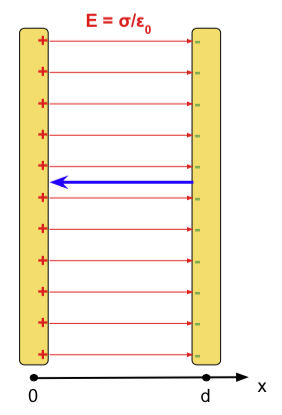
\includegraphics[width=0.99\textwidth]{./images/schematics/parallel_plate_capacitor_path_integral.png}\\
   \end{center}
  \end{column}
  \begin{column}{0.75\textwidth}
    \begin{equation*}
       V = - \int_{d}^{0} \big( E \hat{x} \big) \cdot \Big( dx \hat{x} \Big) \Rightarrow
    \end{equation*}
    \begin{equation*}
      V = - E (\hat{x} \cdot \hat{x}) \int_{d}^{0} dx \Rightarrow
      V =  E d \xRightarrow{E = \frac{\sigma}{\epsilon_0}}
    \end{equation*}
    \begin{equation*}
       {\color{magenta} V =  \frac{\sigma d}{\epsilon_0} }
    \end{equation*}

  \end{column}
\end{columns}

\end{frame}

%
%
%

\begin{frame}{Capacitance of parallel plate capacitor}

\begin{columns}
  \begin{column}{0.30\textwidth}
   \begin{center}
     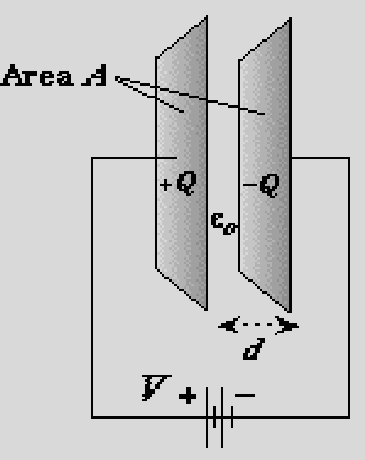
\includegraphics[width=0.80\textwidth]{./images/schematics/parallel_plate_capacitor.png}\\
     \vspace{0.2cm}
     {\scriptsize
       Capacitance (example):\\
       A parallel plate capacitor with plates of area A = 100 mm$^2$ separated by a distance d = 10 mm
       has a capacitance of 0.0885 pF.\\
       If the potential difference between the two plates is 1 V
       this capacitor can hold charge of 0.0885 pC.\\
     }
   \end{center}
  \end{column}
  \begin{column}{0.70\textwidth}
     Using Gauss' law we calculated the field between the two plates:
     \begin{equation*}
         \vec{E} = \frac{\sigma}{\epsilon_0} \hat{x}
     \end{equation*}
     This allowed us to calculate the potential difference between the two plates:
     \begin{equation*}
         V =  \frac{\sigma d}{\epsilon_0}
     \end{equation*}
     Therefore, the capacitance is:
     \begin{equation*}
        C = \frac{Q}{{\Delta}V} = \frac{\sigma A}{\sigma d / \epsilon_0} \Rightarrow {\color{magenta} C = \epsilon_0 \frac{A}{d}}
     \end{equation*}
     Notice that it depends only on the geometrical characteristics of the capacitor (and $\epsilon_0$).
  \end{column}
\end{columns}

\end{frame}



%
% Example
%

{
\problemslide

%
%
%

\begin{frame}{Homework}

Repeat the capacitance calculation for systems with cylindrical
and spherical symmetry, and confirm the answers given below.

\begin{columns}
  \begin{column}{0.60\textwidth}
   \begin{center}
     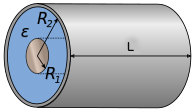
\includegraphics[width=0.75\textwidth]{./images/schematics/capacitors_cylindrical_1.png}\\
     \begin{equation*}
         C = \frac{2 \pi \epsilon L}{ln(R_2/R_1)}
     \end{equation*}
   \end{center}
  \end{column}
  \begin{column}{0.40\textwidth}
   \begin{center}
     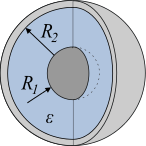
\includegraphics[width=0.75\textwidth]{./images/schematics/capacitors_spherical_1.png}\\
     \begin{equation*}
         C = \frac{4 \pi \epsilon}{\frac{1}{R_1}-\frac{1}{R_2}}
     \end{equation*}
   \end{center}
  \end{column}
\end{columns}

\end{frame}

} % Example



%
%
%

\begin{frame}{Energy stored in a capacitor}

The electric field between the two plates of the parallel plate capacitor is
\begin{equation*}
   {\bf E = \frac{\sigma}{\epsilon_0}}
\end{equation*}

We know there is (electric potential) {\bf energy stored in the electric field}.

\vspace{0.2cm}

It is not difficult to realize that it
{\bf required work to charge the two plates of the capacitor}.
\begin{itemize}
  \item This work became the energy now stored in the electric field.
\end{itemize}

\vspace{0.2cm}

I will {\bf calculate the energy stored in the capacitor}.

\begin{itemize}
{\small
 \item
  This exercise is not very different from the one we did in a previous lecture,
  when we calculated the work done to assemble systems of 2, 3 and N charges, as well as
  continuous distributions of charge.
}
\end{itemize}

\end{frame}


%
%
%

\begin{frame}{Energy stored in a capacitor}

To charge one plate with positive charge and the other with negative charge,
I need to move electrons from one to another.\\

\begin{columns}
  \begin{column}{0.35\textwidth}
   \begin{center}
     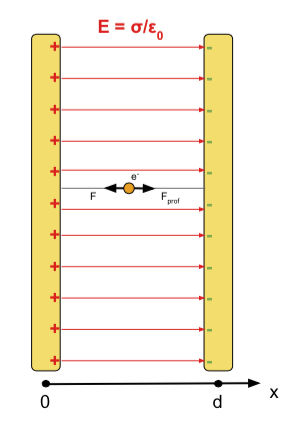
\includegraphics[width=0.99\textwidth]{./images/schematics/parallel_plate_capacitor_work.png}\\
   \end{center}
  \end{column}
  \begin{column}{0.65\textwidth}
  {\small
     Consider I am already some way though that process and that I need to move yet another electron:
      \begin{itemize}
      {\small
         \item There is already some charge on both plates and an electric field is formed between them.
         \item It becomes difficult to move an electron away from the positive (+) and towards the negative (-) plate:
               The electric field exerts a force ($\vec{F}$) on the opposite direction.
         \item I need to exert an equal opposite force ($\vec{F}_{prof}$) to overcome the action of the field.
      }
      \end{itemize}
  }
  \end{column}
\end{columns}

\end{frame}


%
%
%

\begin{frame}{Energy stored in a capacitor}

Assume that I want to move an infinitesimal amount of negative charge -$|{\delta}q|$
from the positive (+) plate at x=0 to the negative (-) plate at x=d.\\

\vspace{0.2cm}

The work I do (against the action of the field) is:
\begin{equation*}
  {\delta}W_{prof} = \int_{+}^{-} \vec{F}_{prof} \cdot d\vec{\ell} = - \int_{+}^{-} \vec{F} \cdot d\vec{\ell}
\end{equation*}
where $\vec{F}$ is the field force and $\vec{F}_{prof}$ is the force that I apply ($\vec{F}_{prof} = - \vec{F}$).\\

\vspace{0.2cm}

The force $\vec{F}$ exerted on the negative charge -$|{\delta}q|$ is given by:
\begin{equation*}
  \vec{F} = -|{\delta}q| \vec{E}
\end{equation*}
Note: $\vec{F}$ and $\vec{E}$ have different directions because the charge is negative.

\end{frame}

%
%
%

\begin{frame}{Energy stored in a capacitor}

Therefore, the work I do can be written as:
\begin{equation*}
  {\delta}W_{prof} =
    |{\delta}q| \int_{+}^{-} \vec{E} \cdot d\vec{\ell} =
    |{\delta}q| \Big( - \int_{-}^{+} \vec{E} \cdot d\vec{\ell} \Big) =
    |{\delta}q| \Big(V_{+} - V_{-} \Big) =
    |{\delta}q| V
\end{equation*}
where V is the difference between the potential of the positive ($V_{+}$) and the negative ($V_{-}$) plate.

The work done move charge Q from one plate to another, is calculate by integrating over $|{\delta}q|$:
\begin{equation*}
  W_{prof} =
     \int {\delta}W_{prof} =
     \int_{0}^{Q}  |{\delta}q| V
\end{equation*}

From the definition of capacitance:
\begin{equation*}
  C = \frac{|q|}{V_{+} - V_{-}} = \frac{|q|}{V} \Rightarrow V = \frac{1}{C} |q|
\end{equation*}

\end{frame}

%
%
%

\begin{frame}{Energy stored in a capacitor}

The work done is:

\begin{equation*}
  W_{prof} = \int_{0}^{Q}  |{\delta}q| V \xRightarrow{V = \frac{1}{C} |q|}
  W_{prof} = \int_{0}^{Q}  \frac{1}{C} |q| |{\delta}q| \Rightarrow
  {\bf W_{prof} = \frac{Q^2}{2C} }
\end{equation*}

Since $C=Q/V$, we can also write the above as:
\begin{equation*}
  W_{prof} = \frac{Q^2}{2C} = \frac{\Big( C V \Big)^2 }{2C} \Rightarrow
  {\bf W_{prof} = \frac{1}{2} C V^2}
\end{equation*}

or, equivalently, as:
\begin{equation*}
  W_{prof} = \frac{Q^2}{2C} = \frac{Q^2}{2\frac{Q}{V}} \Rightarrow
  {\bf W_{prof} = \frac{1}{2} Q V}
\end{equation*}

Again, I note that the work I did ($W_{prof}$) becomes
the {\bf electric potential energy} (U) of the parallel plate capacitor.

\end{frame}

%
%
%

\begin{frame}{Energy stored in a capacitor}

In the previous lecture, we said that the energy stored in the
electric field $\vec{E}$ is the integral, over all space, of $|\vec{E}|^2$.\\
\begin{equation*}
   U = \frac{\epsilon_0}{2} \int_{all\;space} |\vec{E}(\vec{r})|^2  d\tau
\end{equation*}
\vspace{0.1cm}

{\bf Can we show that for the parallel plate capacitor}?\\

\vspace{0.2cm}

{\small
Recall that,
on the previous slide
we calculated that the potential energy U stored in the parallel plate capacitor
(using $W_{prof}$ and U interchangeably):
\begin{equation*}
  U = \frac{1}{2} C V^2
\end{equation*}

And, earlier in the lecture, we calculated
the capacitance C of the parallel plate capacitor, as well as the
potential difference V between its two plates:
\begin{equation*}
  C = \epsilon_0 \frac{A}{d} \;\;\;\;\;\;
  V = \frac{\sigma d}{\epsilon_0}
\end{equation*}
}

\end{frame}

%
%
%

\begin{frame}{Energy stored in a capacitor}

Therefore:

\begin{equation*}
  U = \frac{1}{2} C V^2 \xRightarrow{C = \epsilon_0 \frac{A}{d} \;\;\; V = \frac{\sigma d}{\epsilon_0}}
  U = \frac{1}{2} \Big( \epsilon_0 \frac{A}{d} \Big) \Big( \frac{\sigma d}{\epsilon_0} \Big)^2 \Rightarrow
  U = \frac{\epsilon_0}{2} \Big( A d \Big) \Big( \frac{\sigma}{\epsilon_0} \Big)^2
\end{equation*}

Notice that:
\begin{itemize}
   \item $A{\cdot}d$ is the volume between the two conducting plates
     \begin{itemize}
        \item This is the only volume where $|\vec{E}| \ne 0$
     \end{itemize}
   \item $\sigma/\epsilon_0$ is the electric field between the plates
\end{itemize}

\vspace{0.1cm}

Therefore, the above expression for U can be written as
\begin{equation*}
  U = \frac{\epsilon_0}{2} \Big( Volume \Big) |\vec{E}|^2
\end{equation*}

which is what we sought to show.\\

\end{frame}


%
% Worked example
%

{
\problemslide

%
%
%

\begin{frame}{Worked example}

\begin{blockexmplque}{Question}
The charge centre of a thundercloud, 3 km above ground, carries a charge of 20 C.
Assume the charge centre to be a circle of radius 1 km and model the cloud/ground
system as a parallel plate capacitor. \\
Find:
\begin{enumerate}
   \item The capacitance of the system.
   \item The potential difference between the charge centre and the ground.
   \item The average electric field strength between the cloud and the ground.
   \item The electrical energy stored in the system.
\end{enumerate}
\end{blockexmplque}

\end{frame}

%
%
%

\begin{frame}{Worked example}


\begin{equation*}
   C = \frac{\epsilon_0 A}{d}
      = \frac{(8.854 \times 10^{-12} \; \frac{C^2}{N \cdot m^2}) \cdot \Big( \pi \cdot (1.0 \times 10^3 \; m)^2 \Big)}{3 \times 10^3 \; m}
      = 9.3 \times 10^{-9} \; F
\end{equation*}

\begin{equation*}
   V = \frac{Q}{C}
      = \frac{20 \; C}{9.3 \times 10^{-9} \; F} = 2.2 \times 10^{9} \; V
\end{equation*}

\begin{equation*}
   E = \frac{V}{d}
      = \frac{2.2 \times 10^{9} \; V}{3 \times 10^3 \; m} = 7.3 \times 10^{5} \; V/m
\end{equation*}

\begin{equation*}
   U = \frac{1}{2} Q V
      = \frac{1}{2} (20\; C) (2.2 \times 10^{9} \; V) = 2.2 \times 10^{10} \; J
\end{equation*}

\end{frame}


} % Worked example

%
%
%

\begin{frame}{Dielectrics}

{\bf Another class of materials exists that}, unlike conducting materials, {\bf does not conduct electricity}
(they do not contain free-moving charges).\\
\vspace{0.2cm}
They are called {\bf insulators} or {\bf dielectrics}.\\
\vspace{0.2cm}
Are they {\em "blind"} to the existence of an external electric field?\\
\vspace{0.3cm}

Will see that {\bf this is not the case.}\\

\begin{columns}
  \begin{column}{0.40\textwidth}
   \begin{center}
     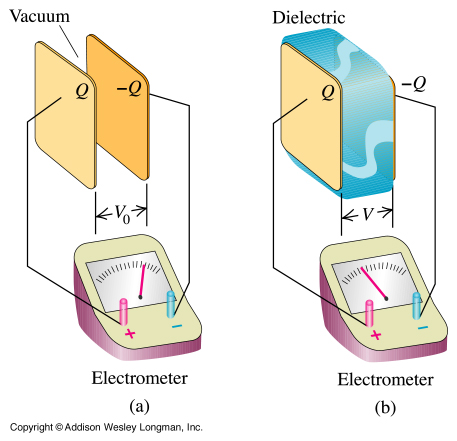
\includegraphics[width=0.95\textwidth]{./images/schematics/parallel_plate_capacitor_with_and_without_dielectric_1.jpg}\\
   \end{center}
  \end{column}
  \begin{column}{0.60\textwidth}
  {\small
    Even from the early days in the development of electromagnetism,
    it was noticed (by Faraday) that {\bf if you insert a dielectric material within a parallel plate capacitor
    its capacitance increases substantially!}\\
    \vspace{0.2cm}
    This means that by inserting a dielectric between the plates
    one {\bf can store the same amount of charge at a much smaller potential difference}.
  }
  \end{column}
\end{columns}

\end{frame}

%
%
%

\begin{frame}{Dielectrics}

Recall that the potential difference V between the two plates is given by
\begin{equation*}
  V = V_{+} - V_{-} = - \int_{-}^{+} \vec{E} \cdot d\vec{\ell}
\end{equation*}

\vspace{0.1cm}

So, by inserting dielectric material within a parallel plate capacitor,
the electric field between the two plates (i.e. within the dielectric) is now much smaller!\\

\vspace{0.2cm}

How is this possible?
\begin{itemize}
{\small
  \item Unlike conductors, the dielectric has no free charges whose redistribution within the
        volume of the material creates an opposing field.
  \item What is the physics mechanism that is responsible for the reduction of the strength
        of the electric field?
}
\end{itemize}

\vspace{0.2cm}

Before we answer the above question, let's examine the {\bf electric dipole}.\\

\end{frame}

%
%
%

\begin{frame}{Electric dipoles and electric dipole moment}

\begin{columns}
  \begin{column}{0.25\textwidth}
   \begin{center}
     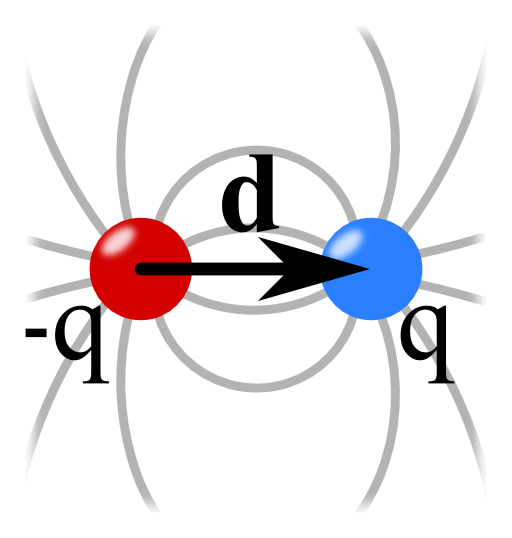
\includegraphics[width=0.95\textwidth]{./images/schematics/electric_dipole_1.png}\\
   \end{center}
  \end{column}
  \begin{column}{0.75\textwidth}
     Let's consider two point charges +q and -q separated by a {\em small distance} d:
     This is an {\bf electric dipole}.\\
     \vspace{0.3cm}
     How small is a "{\em small distance}"? 1 mile? 1 m? 1 mm?
     \begin{itemize}
        \item Small compared with the distances
                 where we are interested to know the field.\\
     \end{itemize}
  \end{column}
\end{columns}

\vspace{0.2cm}
{\bf Dipoles are a very common} configuration in nature.\\

\vspace{0.2cm}
An electric dipole its described by its {\bf electric dipole moment} $\vec{p} = q \vec{d}$\\
\begin{itemize}
  \item The dipole moment is a vector quantity.
  \item Its direction is from the negative to the positive charge.\\
\end{itemize}

The potential field $V(\vec{r})$ due to an {\bf electric dipole} is
\begin{equation*}
   V \approx \frac{1}{4\pi\epsilon_0} \frac{\vec{p} \cdot \hat{r}}{r^2}
\end{equation*}

\end{frame}


%
%
%

\begin{frame}{Examples of electric dipoles in nature (1)}

Consider an unpolarised atom within an external electric field.\\
\begin{itemize}
  \item Initially the centres of gravity of the negative and positive charge distributions coincide.
  \item But, in the presence of an external electric field, the electron cloud and the nucleus are {\em pulled apart}.
\end{itemize}
In the presence of a field, the atom {\bf becomes an electric dipole}.\\
\vspace{0.2cm}
\begin{center}
  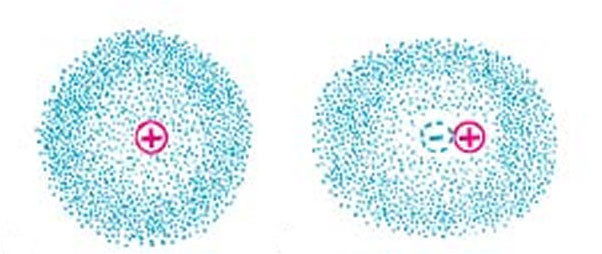
\includegraphics[width=0.75\textwidth]{./images/schematics/dipole_atom_1.jpg}\\
\end{center}

\end{frame}

%
%
%

\begin{frame}{Examples of electric dipoles in nature (2)}

{\bf Complex molecules can be polarised even in the absence of an external electric field}.\\
\vspace{0.1cm}
Perhaps the most common example is the water molecule.\\
\vspace{0.2cm}

\begin{columns}
  \begin{column}{0.50\textwidth}
   \begin{center}
     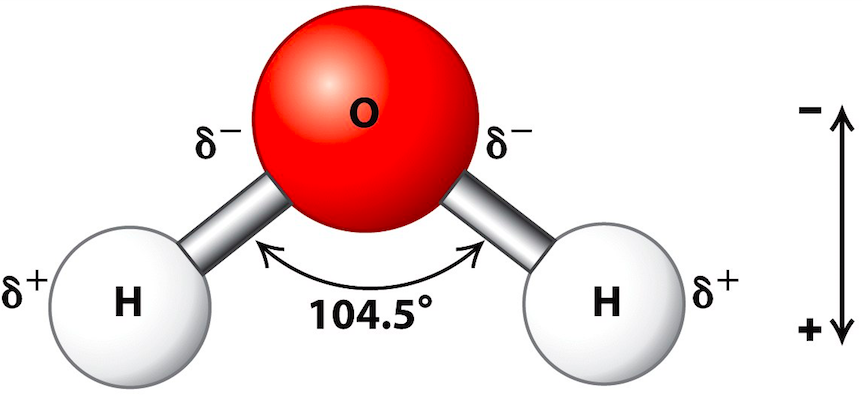
\includegraphics[width=0.98\textwidth]{./images/schematics/dipole_H2O_1.png}\\
   \end{center}
  \end{column}
  \begin{column}{0.50\textwidth}
    \begin{itemize}
    {\small
      \item The 2 H atoms form an angle of 105$^o$ with the O atom.
      \item There is a net negative charge around the O atom.
        \begin{itemize}
        {\scriptsize
            \item Electrons spend more time around the O atom than around the H atoms.
        }
        \end{itemize}
      \item Consequently, there is net positive charge around the two H atoms.\\
    }
    \end{itemize}
  \end{column}
\end{columns}

\vspace{0.4cm}

Although this is more complex configuration than a simple dipole,
when viewed from a distance it is very similar to a dipole.\\

\end{frame}

%
%
%

\begin{frame}{Polar molecules in the presence of an electric field}

In substances with polar molecules, the {\bf electric dipole moments
of the polar molecules are randomly oriented}.\\

\vspace{0.3cm}

\begin{columns}
  \begin{column}{0.40\textwidth}
   \begin{center}
     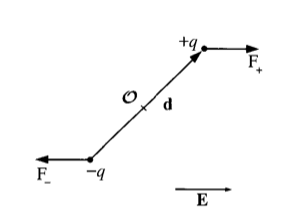
\includegraphics[width=0.80\textwidth]{./images/schematics/electric_dipole_torque_0.png}\\
   \end{center}
  \end{column}
  \begin{column}{0.60\textwidth}
      An external electric field produces a {\bf torque $\vec{T}$ on
      an electric dipole $\vec{p}$}:
      \begin{equation*}
          \vec{T} = \vec{p} \times \vec{E}
      \end{equation*}
  \end{column}
\end{columns}

\vspace{0.3cm}

Therefore, in the presence of an external electric field,
{\bf polar molecules will tend to get aligned along the direction of the field}.

\end{frame}

%
%
%

\begin{frame}{Macroscopic electric polarisation of dielectrics}

The key observations:
\begin{itemize}
 \item An electric field can induce an electric dipole moment in previously unpolarised atoms.
       The dipole moments are aligned with the electric field.
 \item An electric field exerts a torque on polar molecules (molecules with permanent electric
       dipole moment) aligning the previously randomised dipole moment vectors along the
       direction of the field.
\end{itemize}

\vspace{0.2cm}

The dielectric becomes {\bf macroscopically polarised}.\\

\vspace{0.2cm}

The {\bf polarisation} $\vec{P}$ is defined as the
{\bf amount of electric dipole moment per unit volume}.\\

\begin{itemize}
  \item The polarised material creates a field of its own.
  \item This polarisation field opposes the external field that created the polarisation in the first place.
  \item Unlike in conductors, the field cancelation is not complete.
\end{itemize}

\end{frame}

%
%
%

\begin{frame}{Polarization charges}

Let's consider what would happen if the microscopic dipoles were all
perfectly aligned along a direction.

\begin{center}
  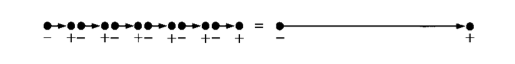
\includegraphics[width=0.80\textwidth]{./images/schematics/polarization_charges.png}\\
\end{center}

The positive charge at the "head" of a dipole cancels the negative charge at the "tail"
of the neighbouring dipole. At the end, the only unbalanced charges appear on the surface.

\vspace{0.2cm}

{\bf A polarised material has a surface charge density} due to unbalanced polarisation charges.\\

\end{frame}


%
%
%

\begin{frame}{Surface density of polarization charge}

{\bf What is the surface charge density} due to polarisation charges?\\

\begin{columns}
  \begin{column}{0.35\textwidth}
   \begin{center}
     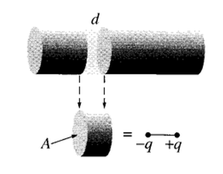
\includegraphics[width=0.85\textwidth]{./images/schematics/polarisation_surface_charge_density_1.png}\\
   \end{center}
  \end{column}
  \begin{column}{0.65\textwidth}
      Consider a cylindrical dielectric, with cross-section A,
      whose axis runs parallel to an external electric field.
      Take a slide of length d: polarisation charge $\pm$q is
      accumulated on the cross-sectional areas.\\
  \end{column}
\end{columns}

Let P be the polarisation. The total electric dipole moment of the slice is:
\begin{equation*}
  P \Big( A \cdot d \Big) = q \cdot d \Rightarrow q = A \cdot P
\end{equation*}

If the surface charge density is ${\sigma}_P$ (charge per area) then:
\begin{equation*}
  q = {\sigma}_P \cdot A
\end{equation*}

Therefore, the charge density is:
\begin{equation*}
  {\color{magenta} {\sigma}_P = P}
\end{equation*}

\end{frame}

%
%
%

\begin{frame}{Surface density of polarization charge}

\begin{columns}
  \begin{column}{0.35\textwidth}
   \begin{center}
     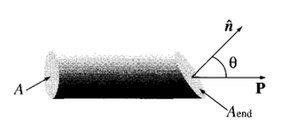
\includegraphics[width=0.95\textwidth]{./images/schematics/polarisation_surface_charge_density_2.png}\\
   \end{center}
  \end{column}
  \begin{column}{0.65\textwidth}
    If the end cap was at an angle $\theta$ with respect to the polarisation vector,
    it would still contain the same amount of charge Q, but the area of the endcap would be larger ($A / cos\theta$)
  \end{column}
\end{columns}

\vspace{0.2cm}

In that case, the charge density would have been
\begin{equation*}
  {\sigma}_P = P cos\theta
\end{equation*}

So the surface density of polarisation charges can be expressed
as the dot product of the polarisation vector $\vec{P}$ with a unit vector $\hat{n}$ normal to the surface
\begin{equation*}
 {\color{magenta} {\sigma}_P = \vec{P} \cdot \hat{n}}
\end{equation*}

\end{frame}

%
%
%

\begin{frame}{Volume density of polarization charge}

{\bf Are the polarisation charges always on the surface?}\\
\vspace{0.1cm}

The answer to this question depends on the alignment of the microscopic dipole moments.
Consider a case where the polarisation field diverges:
\begin{itemize}
{\small
  \item At a point of positive divergence, I have accumulation of negative volume
        (not surface) polarisation charge.
  \item Similarly, negative divergence causes the accumulation of positive polarisation charge.
}
\end{itemize}

\begin{columns}
  \begin{column}{0.35\textwidth}
   \begin{center}
     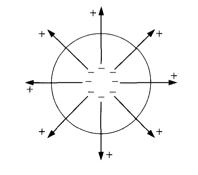
\includegraphics[width=0.95\textwidth]{./images/schematics/divergent_polarization.png}\\
   \end{center}
  \end{column}
  \begin{column}{0.65\textwidth}
     The volume density of polarisation charges can be written as
     \begin{equation*}
       {\color{magenta} {\rho}_P = - \vec{\nabla} \cdot \vec{P}}
     \end{equation*}
     So charge can also accumulate in the volume of an insulator,
     as long as the polarisation field diverges.
  \end{column}
\end{columns}

\end{frame}

%
%
%

\begin{frame}{Electric field produced by a polarized dielectric}

An external electric field $\vec{E}_{0}$
{\bf induces both surface and volume charges} (polarization charges) to a dielectric.\\
\vspace{0.2cm}

The dielectric becomes the {\bf source of a new electric field $\vec{E}_{P}$}.\\
\vspace{0.2cm}

$\vec{E}_{P}$ is the field produced by a surface charge density
$\sigma_P = \vec{P} \cdot \hat{n}$ and a volume charge density $\rho_P = - \vec{\nabla} \cdot \vec{P}$:
\begin{equation*}
 V_P(\vec{r}) = \frac{1}{4\pi\epsilon_0} \oint \frac{1}{r} {\sigma}_P(\vec{r^{\prime}}) dS^{\prime} +
                \frac{1}{4\pi\epsilon_0} \oint \frac{1}{r} {\rho}_P(\vec{r^{\prime}}) d\tau^{\prime}
\end{equation*}
\begin{equation*}
 \vec{E}_{P}(\vec{r}) = - \vec{\nabla} V_P(\vec{r})
\end{equation*}

The total field in the presence of the dielectric is:
\begin{equation*}
 \vec{E}(\vec{r}) = \vec{E}_{0}(\vec{r}) + \vec{E}_{P}(\vec{r})
\end{equation*}

As we mentioned already, $\vec{E}_{P}$ opposes $\vec{E}_{0}$.

\end{frame}

%
%
%

\begin{frame}{Electric field produced by a polarized dielectric}

In order to calculate the total electric field $\vec{E}$,
we need to calculate the field due to induced charges $\vec{E}_P$ and add it to the external field $\vec{E}_0$.\\

To calculate $\vec{E}_P$, we need the surface and volume charge densities:
\begin{equation*}
   {\sigma}_P = \vec{P} \cdot \hat{n} \;\;\;\; and \;\;\;\;
   {\rho}_P = - \vec{\nabla} \cdot \vec{P}
\end{equation*}

Both ${\sigma}_P$ and ${\rho}_P$ depend on the polarisation field $\vec{P}$.
How is it calculated?\\

\begin{columns}
  \begin{column}{0.25\textwidth}
   \begin{center}
     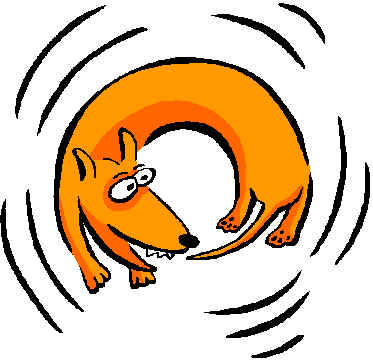
\includegraphics[width=0.90\textwidth]{./images/misc/dog_chasing_tail.jpg}\\
   \end{center}
  \end{column}
  \begin{column}{0.75\textwidth}
    For many materials (called {\bf linear dielectrics}) the polarisation is
    proportional to the total electric field $\vec{E}$ (assuming that $\vec{E}$ is not strong enough)
    \begin{equation*}
       \vec{P} = \chi_{e} \epsilon_0 \vec{E}
    \end{equation*}
  \end{column}
\end{columns}

The factor {\bf $\chi_{e}$ is the electric susceptibility} and depends on the material.\\
The factor $\epsilon_0$ is there mainly so that $\chi_{e}$ becomes dimensionless.\\

\end{frame}

%
%
%

\begin{frame}{Gauss's law in dielectrics}

We will {\bf generalise Gauss's law in the presence of dielectrics}
(where besides free charges we also have induced polarisation charges).\\

\vspace{0.2cm}

Recall Gauss' law (in differential form) in vacuum:
\begin{equation*}
   \vec{\nabla} \cdot \vec{E} = \frac{\rho}{\epsilon_0}
\end{equation*}
where $\rho$ is the total charge density and, now, includes both free ($\rho_f$) and polarisation charges ($\rho_P$):
\begin{equation*}
   \vec{\nabla} \vec{E} = \frac{\rho_f + \rho_P}{\epsilon_0}
\end{equation*}

The density of polarisation charges can be expressed in terms of the polarisation vector, therefore:
\begin{equation*}
   \vec{\nabla} \cdot \vec{E} = \frac{\rho_f - \vec{\nabla} \cdot \vec{P}}{\epsilon_0}
\end{equation*}

\end{frame}

%
%
%

\begin{frame}{Gauss's law in dielectrics}


Collecting the divergences together:

\begin{equation*}
   \vec{\nabla} \cdot \vec{E} = \frac{\rho_f - \vec{\nabla} \cdot \vec{P}}{\epsilon_0} \Rightarrow
   \epsilon_0 \vec{\nabla} \cdot \vec{E} = \rho_f - \vec{\nabla} \cdot \vec{P} \Rightarrow
   \epsilon_0 \vec{\nabla} \cdot \vec{E} + \vec{\nabla} \cdot \vec{P} = \rho_f \Rightarrow
\end{equation*}

\begin{equation*}
   \vec{\nabla} \cdot \Big( \epsilon_0 \vec{E} + \vec{P} \Big) = \rho_f
\end{equation*}

We define the {\bf electric displacement $\vec{D}$} as:
\begin{equation*}
   \vec{D} = \epsilon_0 \vec{E} + \vec{P}
\end{equation*}

In SI, the electric displacement $\vec{D}$ has {\bf units of $C/m^2$}.

\end{frame}

%
%
%

\begin{frame}{Gauss's law in dielectrics}

The electric displacement vector $\vec{D}$ satisfies the differential equation:
\begin{equation*}
   \vec{\nabla} \cdot \vec{D} = \rho_f
\end{equation*}
Notice that $\rho_f$ is the density of {\bf free charges}.\\

\vspace{0.3cm}

This is {\bf Gauss' law}, in differential form, in the presence of dielectrics.\\

\vspace{0.2cm}

We have generalised Gauss's law, taking into account {\bf both free and polarisation charges}.\\

\vspace{0.2cm}

The equivalent integral form can be obtained using Gauss's theorem:
\begin{equation*}
   \oint \vec{D} \cdot d\vec{S} = Q_f
\end{equation*}

Notice that $Q_f$ is the {\bf free charge}.

\end{frame}


%
%
%

\begin{frame}{Gauss's law in dielectrics}

As we have seen, we can then write the
polarization $\vec{P}$ in terms of $\vec{E}$:
\begin{equation*}
  \vec{P} = \chi_{e} \epsilon_0 \vec{E}
\end{equation*}

\vspace{0.3cm}

Now, let's focus on dielectric materials which are:
\begin{itemize}
{\small
  \item {\bf Linear}: $\chi_{e}$ independent of the magnitude of $\vec{E}$
  \item {\bf Isotropic}: $\chi_{e}$ independent of the direction of $\vec{E}$.
  \item {\bf Homogeneous}: $\chi_{e}$ independent of the position.
}
\end{itemize}

Therefore, the electric displacement becomes:
\begin{equation*}
   \vec{D} = \epsilon_0 \vec{E} + \vec{P}
           = \epsilon_0 \vec{E} + \chi_{e} \epsilon_0 \vec{E}
           = \Big( 1 + \chi_{e} \Big) \epsilon_0 \vec{E}
           = \epsilon_{r} \epsilon_0 \vec{E}
\end{equation*}

where $\epsilon_{r} = 1 + \chi_{e}$ is the {\bf relative permittivity} of the dielectric material
(sometimes also called {\bf dielectric constant}).

\end{frame}


%
%
%

\begin{frame}{Gauss's law in dielectrics}

{\small

You probably think that $\vec{D}$ is much like $\vec{E}$: They both obey Gauss's law. \\
\vspace{0.1cm}

{\bf Notice that this is not quite true}.\\
\vspace{0.1cm}

In the previous lecture, we stressed that the divergence of a vector field
is not sufficient to uniquely determine all components of the field.
One also needs the curl of the field.\\
\vspace{0.2cm}

We used that freedom provided by $\vec{\nabla} \times \vec{E} = 0$
to express $\vec{E}$ as the gradient of a scalar field (the potential V).\\
\vspace{0.2cm}

{\bf What is the rotation of $\vec{D}$}?\\
\begin{equation*}
   \vec{\nabla} \times \vec{D} =
   \vec{\nabla} \times \Big( \epsilon_0 \vec{E} + \vec{P} \Big) =
   \epsilon_0  \vec{\nabla} \times \vec{E} + \vec{\nabla} \times \vec{P} \Rightarrow
   \vec{\nabla} \times \vec{D} = \vec{\nabla} \times \vec{P}
\end{equation*}

So, in principle, the curl of $\vec{D}$ is not always 0.
\begin{itemize}
   \item There is no scalar function (potential) whose gradient is $\vec{D}$.
\end{itemize}

Notice that for linear materials:
\begin{equation*}
  \vec{\nabla} \times \vec{P} =
  \vec{\nabla} \times \Big( \chi_{e} \epsilon_0 \vec{E} \Big) =
  \epsilon_{r} \epsilon_0 \vec{\nabla} \times \vec{E} = 0
\end{equation*}

}

\end{frame}

%
%
%

\begin{frame}{Parallel plate capacitor {\em with dielectric}}

Let's consider again the parallel plate capacitor we studied before.\\

\vspace{0.4cm}

\begin{columns}
  \begin{column}{0.45\textwidth}
   \begin{center}
     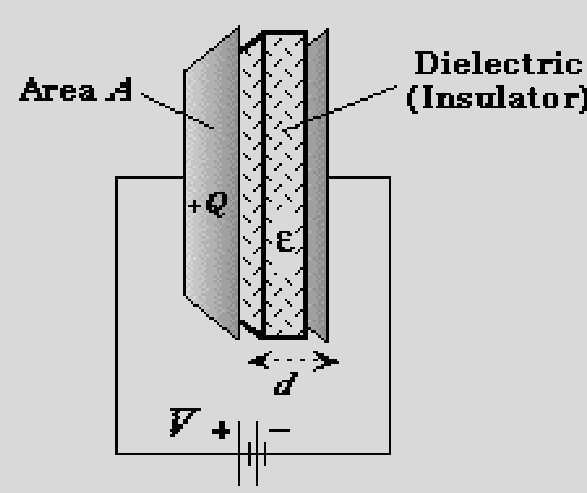
\includegraphics[width=0.95\textwidth]{./images/schematics/parallel_plate_capacitor_dielectric.png}\\
   \end{center}
  \end{column}
  \begin{column}{0.55\textwidth}
    This time, we will examine what happens to its capacity if we {\bf insert a dielectric
    (insulator) within its two oppositely charged plates}.\\
    \vspace{0.2cm}
    We will follow the exact same procedure we followed earlier in this lecture,
    but now we will {\bf use Gauss's law in the presence of dielectrics}.\\
    \begin{equation*}
       \oint \vec{D} \cdot d\vec{S} = Q_f
    \end{equation*}
  \end{column}
\end{columns}

\end{frame}

%
%
%

\begin{frame}{Parallel plate capacitor {\em with dielectric}}

I will use the same Gaussian surface as before and apply Gauss's law in integral form.
Both $\vec{D}$ and $d\vec{S}$ point along $\hat{x}$,
and there is flux only through the right side of the Gaussian surface.

\begin{equation*}
   \oint \vec{D} \cdot d\vec{S} = Q_{f} \Rightarrow D A = Q_{f} \Rightarrow \vec{D} = \frac{Q_{f}}{A} \hat{x}
\end{equation*}

As we have seen the electric displacement $\vec{D}$ is:
\begin{equation*}
   \vec{D} = \epsilon_{r} \epsilon_{0} \vec{E}
\end{equation*}

Therefore the total electric field $\vec{E}$ is:
\begin{equation*}
   \vec{E} = \frac{Q_{f}}{\epsilon_{r} \epsilon_{0} A} \hat{x}
\end{equation*}

\end{frame}

%
%
%

\begin{frame}{Parallel plate capacitor {\em with dielectric}}

The potential difference between the two charged plates is
\begin{equation*}
    V = - \int_{-}^{+} \vec{E} \cdot d\vec{\ell} =  - \int_{d}^{0} \vec{E} \cdot d\vec{\ell}
      = - \int_{d}^{0} \Big( \frac{Q_{f}}{\epsilon_{r} \epsilon_{0} A} \hat{x} \Big) \cdot dl \hat{x} \Rightarrow
      = - \frac{Q_{f}}{\epsilon_{r} \epsilon_{0} A} \int_{d}^{0} dl \Rightarrow
\end{equation*}
\begin{equation*}
    V = \frac{Q_{f} d}{\epsilon_{r} \epsilon_{0} A}
\end{equation*}

Therefore, the capacitance is
\begin{equation*}
       C = \frac{Q_{f}}{{\Delta}V} = \frac{Q_{f}}{\frac{Q_{f} d}{\epsilon_{r} \epsilon_{0} A}} \Rightarrow
  {\bf C = \frac{\epsilon_{r} \epsilon_{0} A}{d} } \Rightarrow
  {\bf C = \epsilon_{r} C_{0}}
\end{equation*}

{\bf In the presence of a dielectric,
the capacitance is multiplied by the relative permittivity $\epsilon_{r}$}.\\

\end{frame}

% ------------------------------------------------------------------------------
% ------------------------------------------------------------------------------

%
% Worked example
%

{
\problemslide


\begin{frame}{Worked example}

\begin{blockexmplque}{Question}

A parallel plate capacitor with a given charge $Q_0$ has an electric field of
$3.2 \times 10^5 \; V/m$ in vacuum and
$2.5 \times 10^5 \; V/m$ when filled with a dielectric.
Find:
\begin{enumerate}
   \item The relative permittivity of the dielectric.
   \item the charge density on the surface of the dielectric.
\end{enumerate}

\end{blockexmplque}

\begin{equation*}
  C_{diel} = \epsilon_r C_0 \xRightarrow{C=Q/V}
 \frac{\cancel{Q_0}}{V_{diel}} = \epsilon_r \frac{\cancel{Q_0}}{V_{0}} \Rightarrow
 \epsilon_r = \frac{V_{0}}{V_{diel}}  \xRightarrow{V = -\int \vec{E} d\vec{\ell}}
\end{equation*}
\begin{equation*}
  \epsilon_r = \frac{E_{0} \cancel{d}}{E_{diel}\cancel{d}} =
                       \frac{3.2 \times 10^5 \; V/m}{2.5 \times 10^5 \; V/m}
  \Rightarrow
  \epsilon_r = 1.28
\end{equation*}
\begin{equation*}
  \chi_e = \epsilon_r - 1 = 1.28 - 1 \Rightarrow \chi_e = 0.28
\end{equation*}
\begin{equation*}
  \sigma_P = P = \chi_e \epsilon_0 E =
      0.28 \cdot (8.854 \times 10^{-12}) \cdot (2.5 \times 10^5) \; C/m^2 = 6.2 \times 10^{-7} C/m^2
\end{equation*}


\end{frame}

} % Worked example

% ------------------------------------------------------------------------------
% ------------------------------------------------------------------------------

%
% Worked example
%

{
\problemslide

\begin{frame}{Worked example}

\begin{blockexmplque}{Question}
A parallel plate capacitor filled with air (for which vacuum is a good approximation in our problem)
has a capacitance of 12.5 $\mu$F and is connected to a power supply which keeps it at constant
potential difference of 24 V. A piece of material with a relative permittivity of 3.75 is placed
between the plates completely filling the space between them.
How much energy is stored in the capacitor before and after the dielectric is inserted?
\end{blockexmplque}
\vspace{0.2cm}

In air (treated as vacuum): $\displaystyle U_0 = \frac{1}{2} C_0 V^2 = 3.6 \; mJ$\\
\vspace{0.2cm}

In dielectric: $\displaystyle U = \frac{1}{2} C V^2 = \frac{1}{2} \epsilon_r C_0 V^2 = 13.5 \; mJ$\\
\vspace{0.2cm}

Therefore: $\displaystyle  {\Delta}U = U - U_0 = 9.9 \; mJ$\\
\vspace{0.4cm}

The energy stored in the capacitor is increased.

\end{frame}

} % Worked example

% ------------------------------------------------------------------------------
% ------------------------------------------------------------------------------

%
% What to remember
%

\renewcommand{\lecturesummarytitle}{Main points to remember }

\renewcommand{\summarizedlecture}{4 }

%
%
%

\begin{frame}{Lecture \summarizedlecture - \lecturesummarytitle}

\begin{itemize}

  \item With regards to electrical properties, there are 2 types of materials
   \begin{itemize}
     \item materials that conduct electricity: {\bf conductors}
     \item materials that do not conduct electricity: {\bf insulators (dielectrics)}
   \end{itemize}

   \vspace{0.2cm}

   \item A conductor is an object or type of material
         which {\bf contains electric charges that are relatively free to move}
  \begin{itemize}
     \item A {\em \bf perfect conductor} has an {\bf unlimited supply of free charges}.
     \item There are no perfect conductors, but many substances come close!
      \begin{itemize}
           \item e.g. the free charge density in copper is 1.8 $\times$ 10$^{10}$ C/$m^3$.
      \end{itemize}
   \end{itemize}

   \vspace{0.2cm}

   \item If we place a {\bf conductor within an external electric field}:
     \begin{itemize}
       \item The electric field vanishes everywhere inside a conductor.
       \item The potential is constant inside a conductor.
       \item Charge accumulates in the surface.
       \item The field on the surface of a conductor has no tangential component.
     \end{itemize}

\end{itemize}

\end{frame}

%
%
%

\begin{frame}{Lecture \summarizedlecture - \lecturesummarytitle (cont'd)}

\begin{itemize}

   \item Capacitance (C) denotes the ability of a body to store electric charge.
             For a system of two conductors, one with charge +Q held at
             potential $V_{+}$ and one with charge -Q held at potential $V_{-}$,
             the capacitance is a positive
             quantity defined as:
      \begin{equation*}
          C = \frac{Q}{V_{+} - V_{-}}
      \end{equation*}
      Its SI unit is the {\bf Farad (F)} defined as one Coulomb per Volt.

   \vspace{0.1cm}

   \item Calculating the capacitance for simple systems:

        \begin{itemize}
         {\small
              \item Use Gauss' law to calculate the electric field $\vec{E}$
                        in terms of the charge Q stored in one of the conductors:
                       $\oint_{S} \vec{E} \cdot d\vec{S} = Q/\epsilon_0$

              \item Once $\vec{E}$ is known, calculate the potential
                        difference V between the two conductors as:
                        $V := {\Delta}V = V_{+} - V_{-} = - \int_{-}^{+} \vec{E} \cdot d\vec{\ell}$

               \item From the known charge Q in the positive conductor and
                         the potential difference V between the conductors,
                         calculate $C = Q/V$
        }
        \end{itemize}

\end{itemize}

\end{frame}


%
%
%

\begin{frame}{Lecture \summarizedlecture - \lecturesummarytitle (cont'd)}

\begin{itemize}

   \item We studied a simple system: The {\bf parallel plate capacitor}

   \item The electric field between the plates was found to be:
      \begin{equation*}
        E = \frac{\sigma}{\epsilon_0}
      \end{equation*}

   \item The parallel plate capacitor has capacitance:
      \begin{equation*}
          C = \epsilon_0 \frac{A}{d}
      \end{equation*}
      It depends only on the geometrical characteristics of the capacitor.

   \item Energy stored in the parallel plate capacitor:
      \begin{equation*}
          U = \frac{Q^2}{2C} \;\;\;\; or \;\;\;\;
          U = \frac{1}{2} C V^2 \;\;\;\; or \;\;\;\;
          U = \frac{1}{2} Q V
      \end{equation*}
      and confirmed that:
      \begin{equation*}
          U = \frac{\epsilon_0}{2} \int_{all\;space} |\vec{E}(\vec{r})|^2  d\tau
      \end{equation*}

\end{itemize}

\end{frame}

%
%
%

\begin{frame}{Lecture \summarizedlecture - \lecturesummarytitle (cont'd)}

\begin{itemize}

   \item  {\bf Electric dipole}:
          Point charges +q and -q at a {\em small distance} d.\\

          \vspace{0.1cm}

   \item  An electric dipole its described by its {\bf electric dipole moment} $\vec{p} = q \vec{d}$\\
          \begin{itemize}
                 \item A vector pointing from the negative to the positive charge
           \end{itemize}

          \vspace{0.1cm}

   \item  An electric dipole creates a potential field V given by
          \begin{equation*}
            V \approx \frac{1}{4\pi\epsilon_0} \frac{\vec{p} \cdot \hat{r}}{r^2}
          \end{equation*}

   \item  An electric field $\vec{E}$ exerts to an electric dipole with moment $\vec{p}$
          a torque $\vec{T} = \vec{p} \times \vec{E}$

          \vspace{0.1cm}

   \item  Electric fields induce dipole moments in the direction of the field (or align
              towards the direction of the field polar molecules with permanent dipole moments)
              and generate macroscopic polarisation.

          \vspace{0.1cm}

   \item  The {\bf polarisation} $\vec{P}$ of a material is defined as the
          {\bf amount of electric dipole moment per unit volume}.\\

\end{itemize}

\end{frame}


%
%
%

\begin{frame}{Lecture \summarizedlecture - \lecturesummarytitle (cont'd)}

\begin{itemize}

   \item  The polarisation induces surface and volume polarisation charges.
          The corresponding densities are
          $\sigma_P = \vec{P} \cdot \hat{n}$ and $\rho_P = - \vec{\nabla} \cdot \vec{P}$

          \vspace{0.1cm}

    \item In the presence of dielectrics,  Gauss's law need to be generalised
          to include both free charges we also have induced polarisation charges:
          \begin{equation*}
             \vec{\nabla} \cdot \Big( \epsilon_0 \vec{E} + \vec{P} \Big) = \rho_f
              \;\;\;\; and \;\;\;\;
              \oint  \Big( \epsilon_0 \vec{E} + \vec{P} \Big) \cdot d\vec{S} = Q_f
          \end{equation*}
          where $\rho_f$ is the free charge density and $Q_f$ the amount of free charge.

          \vspace{0.1cm}

    \item The vector
           $\vec{D} = \epsilon_0 \vec{E} + \vec{P}$ is the electric displacement vector
          \begin{itemize}
             \item In SI, the electric displacement unit is $C/m^2$.
          \end{itemize}

          \vspace{0.1cm}

    \item For {\bf linear dielectrics},
              $\vec{P} = \chi_{e} \epsilon_0 \vec{E}$ and, therefore,
              $\vec{D} = \epsilon_r \epsilon_0 \vec{E}$,
              where
              $\chi_{e}$ is the electric susceptibility of the material and
              $\epsilon_r = 1 + \chi_e$ is the relative permittivity (dielectric constant).

 \item A dielectric with relative permittivity $\epsilon_r$ inserted
         between the plates of a parallel plate capacitor, increases
         its capacitance by a factor of $\epsilon_r$.

\end{itemize}

\end{frame}

%
%
%

\begin{frame}{Maxwell's equation we know so far}

In vacuum (static case):

\begin{center}
 {
  \begin{table}[H]
    \begin{tabular}{|l|c|c|}
      \hline
          & {\it Integral form} & {\it Differential form} \\
      \hline
      {\bf Gauss's law} &
        $\oint \vec{E} \cdot d\vec{S} = Q_{enclosed} / \epsilon_0$ &
        $\vec{\nabla} \cdot \vec{E} = \rho / \epsilon_0$ \\

      {\bf Circuital law} &
        $\oint \vec{E} \cdot d\vec{\ell} = 0$ &
        $\vec{\nabla} \times \vec{E} = 0$ \\
      \hline
    \end{tabular}
  \end{table}
 }
\end{center}

In the presence of materials (static case):

\begin{center}
 {
  \begin{table}[H]
    \begin{tabular}{|l|c|c|}
      \hline
          & {\it Integral form} & {\it Differential form} \\
      \hline
      {\bf Gauss's law} &
        $\oint \vec{D} d\vec{S} = Q_{enclosed; free}$ &
        $\vec{\nabla} \cdot \vec{D} = \rho_{free}$ \\

      {\bf Circuital law} &
        $\oint \vec{E} d\vec{\ell} = 0$ &
        $\vec{\nabla} \times \vec{E} = 0$ \\
      \hline
    \end{tabular}
  \end{table}
 }
\end{center}

\end{frame}


%
% Plan for the next lecture
%

\begin{frame}{At the next lecture (Lecture \nextlecture)}

\begin{itemize}
\item Electric current.
\item Magnetic phenomena.
\item Electric charge inside a magnetic field.
\item Cyclotron motion.
\item Magnetic force on an electric current.
\item The Biot-Savart law.
\item Magnetic field around a straight wire.
\end{itemize}

\end{frame}

%
% Optional reading
%



% ------------------------------------------------------------------------------
% ------------------------------------------------------------------------------

%
% Optional reading
%

\begin{frame}[plain,c]
\begin{center}
{\Huge \bf Optional reading for Lecture \thislecture}
\end{center}
\end{frame}


%
%
%

\begin{frame}{Electric dipole field}

\begin{columns}
  \begin{column}{0.20\textwidth}
   \begin{center}
     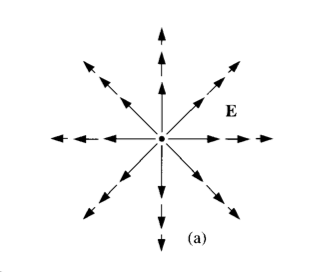
\includegraphics[width=0.99\textwidth]{./images/schematics/electric_field_pos_point_charge.png}\\
   \end{center}
  \end{column}
  \begin{column}{0.80\textwidth}
     As we know, the potential field $V(\vec{r})$ due to an
     {\bf electric monopole} (i.e. a point charge q) has an $1/r$ dependence:
     \begin{equation*}
         V = \frac{1}{4\pi\epsilon_0} \frac{q}{r}
     \end{equation*}
     Consequently, its electric field $\vec{E}(\vec{r})$ ($\vec{E} = -\vec{\nabla}V$)
     has an $1/r^2$ dependence.
  \end{column}
\end{columns}

\vspace{0.3cm}

\begin{columns}
  \begin{column}{0.80\textwidth}
     We will see that the potential field $V(\vec{r})$ due to an {\bf electric dipole} is
     \begin{equation*}
        {\bf V \approx \frac{1}{4\pi\epsilon_0} \frac{\vec{p} \hat{r}}{r^2} }
     \end{equation*}
     Therefore, it falls off as $1/r^2$, faster than the monopole potential.
     Consequently, the dipole electric field $\vec{E}(\vec{r})$
     has an $1/r^3$ dependence.
  \end{column}
  \begin{column}{0.20\textwidth}
   \begin{center}
     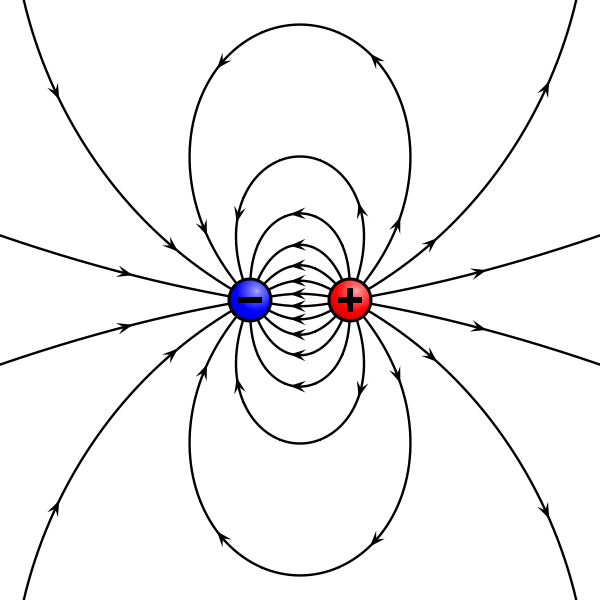
\includegraphics[width=0.90\textwidth]{./images/schematics/electric_dipole_field_lines_2.png}\\
   \end{center}
  \end{column}
\end{columns}

\end{frame}


%
%
%

\begin{frame}{Calculating the electric dipole field}

As we know, the potential field due to a single charge q is given by:
\begin{equation*}
  V = \frac{1}{4\pi\epsilon_0} \frac{q}{r}
\end{equation*}

\vspace{0.1cm}

\begin{columns}
  \begin{column}{0.25\textwidth}
   \begin{center}
     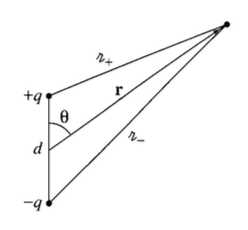
\includegraphics[width=0.95\textwidth]{./images/schematics/electric_dipole_0.png}\\
   \end{center}
  \end{column}
  \begin{column}{0.75\textwidth}
    Now, I have 2 charges: a positive and a negative one. The superposition principle applies.
    The potential at a distance r from the centre of the dipole is:
    \begin{equation*}
      V = \frac{1}{4\pi\epsilon_0} \Big( \frac{q}{r_{+}} - \frac{q}{r_{-}} \Big)
    \end{equation*}
  \end{column}
\end{columns}

\vspace{0.1cm}

I need to express $r_{+}$ and $r_{-}$ in terms of r.
From the law of cosines (generalisation of the Pythagorean theorem):
\begin{equation*}
  r_{+}^{2} = r^{2} + (d/2)^{2} - r \cdot d \cdot cos\theta
            = r^{2} \Big( 1 - \frac{d}{r} cos\theta + \frac{d^2}{4r^2} \Big) \xRightarrow{r>>d}
\end{equation*}
\begin{equation*}
   r_{+}^{2} \approx r^{2} \Big( 1 - \frac{d}{r} cos\theta \Big)
\end{equation*}

\end{frame}

%
%
%

\begin{frame}{Calculating the electric dipole field}

For $r_{-}$, the expressions are similar but involves $cos(\pi - \theta) = -cos\theta$ and,
therefore, there is an extra minus sign.
\begin{equation*}
   r_{-}^{2} \approx r^{2} \Big( 1 + \frac{d}{r} cos\theta \Big)
\end{equation*}

For convenience let me rename the small term involving d/r as $\epsilon$:
\begin{equation*}
  \frac{d}{r} cos\theta = \epsilon
\end{equation*}

We have that
\begin{equation*}
   r_{+}^{2} \approx r^{2} (1 - \epsilon) \Rightarrow
   r_{+} \approx r (1 - \epsilon)^{1/2} \Rightarrow
   \frac{1}{r_{+}} \approx \frac{1}{r} (1 - \epsilon)^{-1/2} \Rightarrow
   \frac{1}{r_{+}} \approx \frac{1}{r} (1 + \frac{1}{2}\epsilon)
\end{equation*}

and, similarly
\begin{equation*}
   \frac{1}{r_{-}} \approx \frac{1}{r} (1 - \frac{1}{2}\epsilon)
\end{equation*}

\end{frame}

%
%
%

\begin{frame}{Calculating the electric dipole field}

Therefore
\begin{equation*}
  \frac{1}{r_{+}} - \frac{1}{r_{-}} \approx
    \Big( \frac{1}{r} (1 + \frac{1}{2}\epsilon) \Big) -
    \Big( \frac{1}{r} (1 - \frac{1}{2}\epsilon) \Big) =
    \frac{1}{r} \epsilon \xRightarrow{\epsilon = \frac{d}{r} cos\theta}
\end{equation*}
\begin{equation*}
  \frac{1}{r_{+}} - \frac{1}{r_{-}} \approx \frac{d}{r^2} cos\theta
\end{equation*}

The electric dipole potential is given by
\begin{equation*}
  V = \frac{1}{4\pi\epsilon_0} \Big( \frac{q}{r_{+}} - \frac{q}{r_{-}} \Big) \Rightarrow
  V \approx \frac{1}{4\pi\epsilon_0} \frac{q d cos\theta}{r^2} \Rightarrow
\end{equation*}
\begin{equation*}
  V \approx \frac{1}{4\pi\epsilon_0} \frac{\vec{p} \cdot \hat{r}}{r^2}
\end{equation*}

So the potential of a dipole falls off as $1/r^2$ ($1/r$ for a monopole).\\
Consequently, the electric field of a dipole falls off as $1/r^3$.\\

\end{frame}

% ------------------------------------------------------------------------------

%
%
%

\begin{frame}{The {\em multipole} expansion}

\begin{columns}
  \begin{column}{0.30\textwidth}
   \begin{center}
     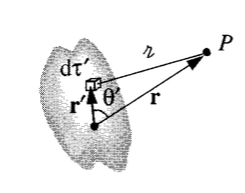
\includegraphics[width=0.99\textwidth]{./images/schematics/continuous_charge_distribution_1.png}\\
   \end{center}
  \end{column}
  \begin{column}{0.70\textwidth}
    For an {\bf arbitrary charge distribution} characterised by a density $\rho$
    the potential can be expanded to:
    \begin{equation*}
      V(r) = \frac{1}{4\pi\epsilon_0} \sum_{n=0}^{\infty} \frac{1}{r^{n+1}}
        \int_{vol} (r^{\prime})^{n} P_{n}(cos\theta^{\prime}) \rho(\vec{r^{\prime}}) d{\tau}^{\prime}
    \end{equation*}
    where $\theta^{\prime}$ is the angle between $\vec{r}$ and $\vec{r^{\prime}}$.
    Notice that there is no r dependence in the integral.\\
  \end{column}
\end{columns}

\vspace{0.3cm}

This is called the {\bf multipole expansion}.
\begin{itemize}
{\small
  \item The first ($1/r$) term is the {\bf monopole} term
  \item The second ($1/r^2$) term is the {\bf dipole} term
  \item $1/r^3$ term: {\bf quadruple} term
  \item $1/r^4$ term: {\bf octopole} term
  \item ...
}
\end{itemize}

\end{frame}

% ------------------------------------------------------------------------------

%
% Worked example : The not-so-parallel plate capacitor
%

{
\problemslide

\begin{frame}{Worked example: The not-so-parallel plate capacitor}

  \begin{blockexmplque}{Question}
  In the figure below, you are given the not-so-parallel plate capacitor.
  \begin{itemize}
    \item
     Neglecting edge effects, when a voltage difference $V_0$ is placed
     across the two conductors, find the potetial everywhere between the plates.
    \item
     When the wedge is filled with a medium of dielectric constant $\epsilon$,
     find the capacitance of the system in terms of the constants given.
  \end{itemize}
  \begin{center}
    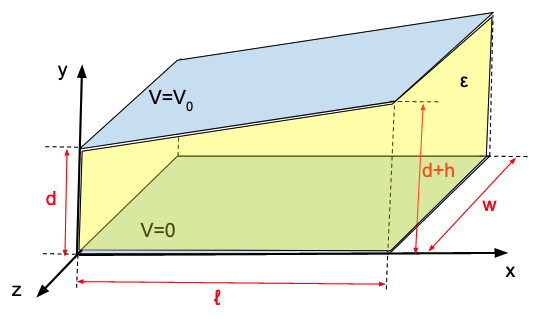
\includegraphics[width=0.60\textwidth]{./images/problems/lect4_not_so_parallel_plane_capacitor_1.png}\\
  \end{center}
  \end{blockexmplque}

\end{frame}

%
%
%

\begin{frame}{Worked example: The not-so-parallel plate capacitor}

Neglecting edge effects, the problem is a two-dimensional one.\\
\vspace{0.1cm}
Symmetry dictates that the electric field is parallel to the $xy$ plane
and it is {\em independent} of $z$.\\
\vspace{0.1cm}
A convenient coordinate system for our analysis is $O^\prime (x^\prime, y^\prime, z^\prime)$
which is shifted from $O (x, y, z)$ by a distance $\ell^\prime$ along the $x$ axis,
so imaginary extrapolations of the capacitor plates
intersect at $x^\prime=0$, as shown below.

\begin{center}
  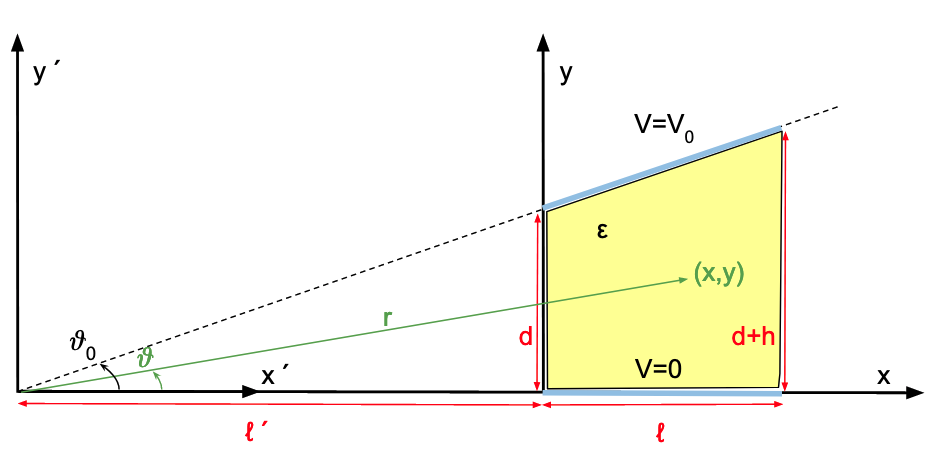
\includegraphics[width=0.80\textwidth]{./images/problems/lect4_not_so_parallel_plane_capacitor_2.png}\\
\end{center}

\end{frame}


%
%
%

\begin{frame}{Worked example: The not-so-parallel plate capacitor}

The quantities $\ell^\prime$, $\theta_0$, $\theta$ and $r$ introduced above (see schematic)
can be easily related to the given quantities $\ell$, $d$, $h$ and the coordinates $x,y$
of a point within the capacitor in the original coordinate system ($O$).

  \begin{equation*}
    tan\theta_0 = \frac{d+h}{\ell+\ell^\prime} = \frac{d}{\ell^\prime} \Rightarrow
     \ell^\prime = \ell \frac{d}{h}
  \end{equation*}

  \begin{equation*}
    tan\theta_0 = \frac{d}{\ell^\prime} = \frac{\cancel{d}}{\ell \frac{\cancel{d}}{h}} \Rightarrow
    \theta_0 = arctan\Big(\frac{h}{\ell}\Big)
  \end{equation*}

  \begin{equation*}
    tan\theta = \frac{y}{x+\ell^\prime} = \frac{y}{x+\ell \frac{d}{h}} \Rightarrow
    \theta = arctan\Big(\frac{y}{x+\ell \frac{d}{h}}\Big)
  \end{equation*}

  \begin{equation*}
    cos\theta = \frac{x+\ell^\prime}{r} = \frac{x+\ell \frac{d}{h}}{r} \xRightarrow{\; cos\theta \approx 1 \;}
    r = x + \ell \frac{d}{h}
  \end{equation*}

\end{frame}

%
%
%

\begin{frame}{Worked example: The not-so-parallel plate capacitor}

The potetial between the plates can be found by solving Poisson's equation

  \begin{equation*}
    \vec{\nabla}^{2} V = \frac{\rho}{\epsilon_0} \xRightarrow{\rho=0}
    \vec{\nabla}^{2} V = 0
  \end{equation*}

In polar coordinates, this is written as

  \begin{equation*}
    \frac{1}{r^2} \frac{d^2V(\theta)}{d\theta} = 0 \Rightarrow
    \frac{d^2V(\theta)}{d\theta} = 0
  \end{equation*}

\vspace{0.2cm}

The equation has the following solution

  \begin{equation*}
    V(\theta) = A + B \theta
  \end{equation*}

The costants $A, B$ can be derived from the boundary conditions

  \begin{equation*}
    V(\theta = 0) = 0 \Rightarrow A = 0
  \end{equation*}

  \begin{equation*}
    V(\theta = \theta_0) = V_0 \xRightarrow{A = 0}
    B \theta_0 = V_0 \Rightarrow B = \frac{V_0}{\theta_0}
  \end{equation*}

\end{frame}

%
%
%

\begin{frame}{Worked example: The not-so-parallel plate capacitor}

Therefore, the solution $V(\theta)$ is given by

  \begin{equation*}
    V(\theta) =  \frac{V_0}{\theta_0} \theta
  \end{equation*}

Using the expression for $\theta_0$ that was derived previously,
$V(\theta)$ can be written as

  \begin{equation*}
    V(\theta) =  \frac{V_0}{arctan\Big(\frac{h}{\ell}\Big)} \theta
  \end{equation*}

In terms of coordinates $x,y$ in the original coordinate system ($O$),
the potential can be expressed as

  \begin{equation*}
    V(x,y) =  \frac{V_0}{arctan\Big(\frac{h}{\ell}\Big)}
     \arctan\Big(\frac{y}{x+\ell \frac{d}{h}}\Big)
  \end{equation*}

\end{frame}

%
%
%

\begin{frame}{Worked example: The not-so-parallel plate capacitor}

The capacitance of the system will be calculated from
  \begin{equation*}
    C = \frac{|Q|}{|V_0|}
  \end{equation*}

where the unknown charge $Q$ can be estimated from
  \begin{equation*}
    Q = \oint \vec{D} \cdot d\vec{S}
  \end{equation*}

The field $\vec{D}$ is related to electric field $\vec{E}$,
and therefore the potential V, as
  \begin{equation*}
    \vec{D} = \epsilon \vec{E} \xRightarrow{\vec{E} = -\vec{\nabla}V}
    \vec{D} = -\epsilon \vec{\nabla}V
  \end{equation*}

Therefore
  \begin{equation*}
    \vec{D} =
      -\epsilon \frac{1}{r} \frac{\partial V}{\partial \theta} \hat{\theta}
      \xRightarrow{\;V =  \frac{V_0}{\theta_0} \theta \;}
    \vec{D} = - \frac{1}{r} \frac{\epsilon V_0}{\theta_0} \hat{\theta}
  \end{equation*}

\end{frame}

%
%
%

\begin{frame}{Worked example: The not-so-parallel plate capacitor}

Using the above expression for $\vec{D}$, $Q$ is calculated as
  \begin{equation*}
    Q = \oint \vec{D} \cdot d\vec{S} = \oint D dS
     \xRightarrow{\; dS = w dx, \; D = - \frac{1}{r} \frac{\epsilon V_0}{\theta_0} \;}
     Q = -\frac{w \epsilon V_0}{\theta_0} \int_{0}^{\ell} \frac{1}{r} dx
      \xRightarrow{\; r = x + \ell \frac{d}{h} \;}
  \end{equation*}

  \begin{equation*}
    Q = -\frac{w \epsilon V_0}{\theta_0} \int_{0}^{\ell} \frac{1}{x + \ell \frac{d}{h}} dx =
        -\frac{w \epsilon V_0}{\theta_0} ln(x + \ell \frac{d}{h}) \Big\rvert_{0}^{\ell} \Rightarrow
  \end{equation*}

  \begin{equation*}
    Q = -\frac{w \epsilon V_0}{\theta_0} ln \frac{d + h}{d}
    \xRightarrow{\theta_0 = arctan\Big(\frac{h}{\ell}\Big)}
    Q = -\frac{w \epsilon V_0}{arctan\Big(\frac{h}{\ell}\Big)} ln \Big(\frac{d + h}{d}\Big)
  \end{equation*}

Therefore
  \begin{equation*}
    C = \frac{|Q|}{|V_0|} =
      \frac{w \epsilon}{arctan\Big(\frac{h}{\ell}\Big)} ln \Big(\frac{d + h}{d}\Big)
  \end{equation*}

\end{frame}


} % Worked example

% ------------------------------------------------------------------------------

%
% Worked example : Pulling a dielectric out of a capacitor
%

{
\problemslide

\begin{frame}{Worked example: Pulling a dielectric out of a capacitor}

  \begin{blockexmplque}{Question}
  A cylindrical capacitor of length $L$ consists of an inner metallic wire
  of radius $a$, and a thin outer metallic shell of radius $b$.
  The space in between is filled with a dielectric with permittivity $\epsilon$.\\
  As we have seen in the workshops, if edge effects are ignored,
  the capacitance $C$ of the cylindrical
  capacitor is given by
  \begin{equation*}
    C = \frac{2\pi \epsilon L}{ln(b/a)}.
  \end{equation*}
  \vspace{0.2cm}
  Suppose that the dielectric is pulled partly out of the capacitor,
  and that the capacitor is connected to a battery of electromotive force $V$.
  \begin{enumerate}
  \item
  Find the force necessary to hold the dielectric in this position.
  \item
  In which direction must the force be applied?\\
  \end{enumerate}
  \end{blockexmplque}

\end{frame}

%
%
%

\begin{frame}{Worked example: Pulling a dielectric out of a capacitor}

  \begin{center}
    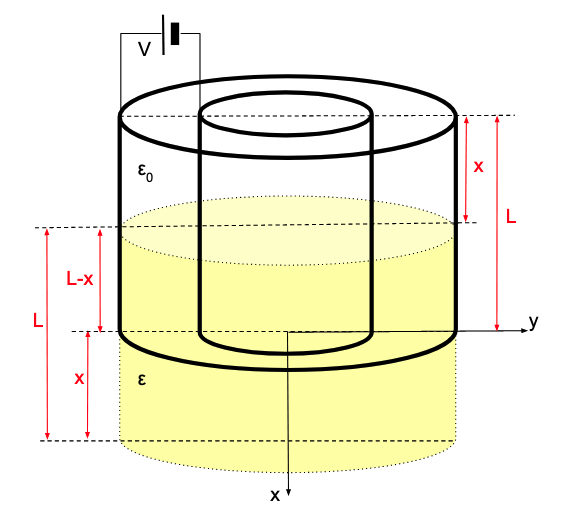
\includegraphics[width=0.67\textwidth]{./images/problems/lect4_pulling_dielectric_out_of_capacitor_1.png}\\
  \end{center}

\end{frame}

%
%
%

\begin{frame}{Worked example: Pulling a dielectric out of a capacitor}

  If the dielectric is pulled out of the cylindrical capacitor by a length $x$,
  then length $L-x$ remains inside the capacitor.

  The part of the capacitor with length $x$ that does not have a dielectric
  has capacitance $C_1$ given by
  \begin{equation*}
    C_1 = \frac{2\pi \epsilon_0 x}{ln(b/a)}
  \end{equation*}
  whereas the part of the capacitor with length $L-x$ that does have a
  dielectric has a capacitance $C_2$ given by
  \begin{equation*}
    C_2 = \frac{2\pi \epsilon (L-x)}{ln(b/a)}.
  \end{equation*}

  Those two capacitors have a common potential difference across the
  inner and outer conductors (connected parallel) and, therefore, the
  combined capacitance $C$ is
  \begin{equation*}
    C = C_1 + C2 =
     \frac{2\pi \epsilon_0 x}{ln(b/a)} +
     \frac{2\pi \epsilon (L-x)}{ln(b/a)} =
     \frac{2\pi \epsilon}{ln(b/a)}
         \Big(L + (\frac{\epsilon_0}{\epsilon}-1) x \Big)
  \end{equation*}

\end{frame}

%
%
%

\begin{frame}{Worked example: Pulling a dielectric out of a capacitor}

  The work provided by the battery as it charges the capacitor
  becomes energy stored in the capacitor and mechanical work of
  the force $F$ that moves the dielectric with respect to the capacitor.
  We can write
  \begin{equation*}
    dW_{battery} = dU_{capacitor} + dW_{mechanical} \Rightarrow
  \end{equation*}
  \begin{equation*}
    V dQ = d\Big(\frac{1}{2}CV^2\Big) + F dx
  \end{equation*}
  Since $V$ is constant, the above can be written as
  \begin{equation*}
    V dQ = \frac{1}{2}V^2 dC + F dx
  \end{equation*}
  Using the definition of capacitance, $C = \frac{Q}{V}$, we can write
  \begin{equation*}
    dC = \frac{dQ}{V} \Rightarrow V^2 dC = V dQ
  \end{equation*}
  From all the above, we obtain
  \begin{equation*}
    V^2 dC = \frac{1}{2}V^2 dC + F dx \Rightarrow
    \frac{1}{2}V^2 dC = F dx
  \end{equation*}

\end{frame}

%
%
%

\begin{frame}{Worked example: Pulling a dielectric out of a capacitor}

  As the dielectric exits the capacitor, $x$ increases
  and, therefore, $dx > 0$.

  When $x$ increases we expect the capacitance $C$ to decrease.
  Given that $\epsilon_0/\epsilon < 1$,
  this can be easily deduced from the expression for $C$,
  \begin{equation*}
    C =
     \frac{2\pi \epsilon}{ln(b/a)}
         \Big(L + (\frac{\epsilon_0}{\epsilon}-1) x \Big).
  \end{equation*}
  Therefore, for $dx > 0$, $dC < 0$.
  Considering this and observing the expression
  \begin{equation*}
    \frac{1}{2}V^2 dC = F dx,
  \end{equation*}
  we see that the term $F dx$ needs to be negative.
  Therefore, for $dx > 0$ (direction of exiting the capacitor),
  the direction of the force on the dielectric is opposite,
  and the dielectric is pulled into the capacitor.

  If we wanted to hold the dielectric in a fixed position, we would
  need to apply an opposite force $\vec{F^\prime}(=-\vec{F})$,
  pointing {\em away} from the capacitor.

\end{frame}

%
%
%

\begin{frame}{Worked example: Pulling a dielectric out of a capacitor}

  The magnitude of my force $F^\prime=F$
  \begin{equation*}
    \frac{1}{2}V^2 dC = F dx \Rightarrow
    F = \frac{1}{2}V^2 \frac{dC}{dx}
  \end{equation*}

  Differentiating the expression for $C$ we derived earlier, we find
  \begin{equation*}
    \frac{dC}{dx} = \frac{2\pi \epsilon}{ln(b/a)}
        \Big(\frac{\epsilon_0}{\epsilon}-1\Big)
  \end{equation*}

  Thefore, the magnitude of the force is given by
  \begin{equation*}
    F = \frac{1}{2}V^2 \frac{2\pi \epsilon}{ln(b/a)}
     \Big(\frac{\epsilon_0}{\epsilon}-1\Big) \Rightarrow
    F = \frac{\pi \epsilon V^2}{ln(b/a)}
      \Big(\frac{\epsilon_0}{\epsilon}-1\Big)
  \end{equation*}

\end{frame}

} % Worked example

% ------------------------------------------------------------------------------

%
% Worked example : Spherical capacitor with inhomogeneous dielectric
%

{
\problemslide

\begin{frame}{Worked example: Cylindrical and spherical capacitors}

  \begin{blockexmplque}{Question}
  Calculate the capacitance of a cylindrical and a spherical capacitor.\\
  \begin{columns}
    \begin{column}{0.60\textwidth}
     \begin{center}
       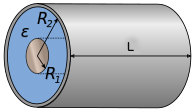
\includegraphics[width=0.75\textwidth]{./images/schematics/capacitors_cylindrical_1.png}\\
       \begin{equation*}
           C = \frac{2 \pi \epsilon L}{ln(R_2/R_1)}
       \end{equation*}
     \end{center}
    \end{column}
    \begin{column}{0.40\textwidth}
     \begin{center}
       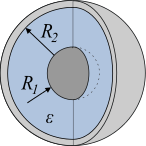
\includegraphics[width=0.75\textwidth]{./images/schematics/capacitors_spherical_1.png}\\
       \begin{equation*}
           C = \frac{4 \pi \epsilon}{\frac{1}{R_1}-\frac{1}{R_2}}
       \end{equation*}
     \end{center}
    \end{column}
  \end{columns}
  \end{blockexmplque}

\end{frame}

%
%
%

\begin{frame}{Worked example: Cylindrical and spherical capacitors}

  %-----------
  % cylindrical
  %-----------

  As a Gaussian surface, for the calculation for a cylindrical capacitor,
  we choose a cylinder of length $L$
  and radius $\rho$ ($R_1$ $\le$ $\rho$ $\le$ $R_2$), closed by end caps.
  It is coaxial with the cylinders of radii $R_1$ and $R_2$ and
  encloses the central cylinder and
  thus also the charge $Q$ on that cylinder.
  Let's assume, without loss of generality, that the inner conductor is
  positively charged and the outer conductor is negatively charged.

  From Gauss' law:
  \begin{equation*}
    \Phi_E = Q/\epsilon_0 \Rightarrow
    \oint_{S} \vec{E} \cdot d\vec{S} = Q/\epsilon_0
  \end{equation*}

  The electric field $\vec{E}$
  is collinear with the normal to the Gaussian surface and, due to
  cylindrical symmetry, it has the same magnitude everywhere on that
  surface. There is no electric flux through the end caps.\\
  The overall flux through the closed Gaussian surface is:
  \begin{equation*}
    \oint_{S} \vec{E} \cdot d\vec{S} =
    \oint_{S} E \cdot dS =
    E \oint_{S} dS =
    E S = E (2\pi \rho L)
  \end{equation*}

\end{frame}

%
%
%

\begin{frame}{Worked example: Cylindrical and spherical capacitors}

  Therefore:
  \begin{equation*}
    E (2\pi \rho L) = Q/\epsilon_0 \Rightarrow
    E = \frac{Q}{2\pi \epsilon_0 L \rho}
  \end{equation*}

  In vector form the electric field is written as:
  \begin{equation*}
    \vec{E} = \frac{Q}{2\pi \epsilon_0 L \rho} \cdot \hat{\rho}
  \end{equation*}
  where $\hat{\rho}$ is the axial radial unit vector of the cylindrical
  coordinate system used (it is perpendicular to the axis of the
  two cylindrical conductors and it points outwards).\\

  The potential difference $V$ between the positively and negatively
  charged conductors is:
  \begin{equation*}
      V := V_{+} - V_{-} = - \int_{-}^{+} \vec{E} \cdot d\vec{\ell}
  \end{equation*}

  This integral is path-independent.
  The integral is simplified if $\vec{E}$ and $d\vec{\ell}$ are colinear.
  Since the electric field points along  $\hat{\rho}$, we chose
  $d\vec{\ell} = d\rho \cdot \hat{\rho}$.\\

\end{frame}

%
%
%

\begin{frame}{Worked example: Cylindrical and spherical capacitors}

  Therefore:
  \begin{equation*}
      V = - \frac{Q}{2\pi \epsilon_0 L} \int_{R_2}^{R_1} \frac{d\rho}{\rho}
  \end{equation*}

  \begin{equation*}
        = -  \frac{Q}{2\pi \epsilon_0 L} ln(\rho) \rvert_{R_2}^{R_1} =
          - \frac{Q}{2\pi \epsilon_0 L}  (ln R_1 - ln R_2) =
            \frac{Q}{2\pi \epsilon_0 L}  (ln R_2 - ln R_1) \Rightarrow
  \end{equation*}

  \begin{equation*}
        V = \frac{Q}{2\pi \epsilon_0 L}  ln(R_2/R_1)
  \end{equation*}

  Therefore, the capacitance of a cylindrical capacitor is given by:
  \begin{equation*}
      C = \frac{Q}{V} = \frac{Q}{\frac{Q}{2\pi \epsilon_0 L}  ln(R_2/R_1)} =
             2\pi \epsilon_0 \frac{L}{ln(R_2/R_1)}
  \end{equation*}

\end{frame}

%
%
%

\begin{frame}{Worked example: Cylindrical and spherical capacitors}

  %-----------
  % spherical
  %-----------

  As a Gaussian surface, for the calculation for a spherical capacitor,
  we choose a sphere of radius $r$ ($R_1$ $\le$ $r$ $\le$ $R_2$)
  which is concentric with the spherical shells of radii $R_1$ and $R_2$.
  Let's assume, without loss of generality, that the inner conductor is
  positively charged and the outer conductor is negatively charged.

  From Gauss' law:
  \begin{equation*}
    \Phi_E = Q/\epsilon_0 \Rightarrow
    \oint_{S} \vec{E} \cdot d\vec{S} = Q/\epsilon_0
  \end{equation*}

  The electric field $\vec{E}$
  is collinear with the normal to the chosen Gaussian surface and, due to
  spherical symmetry, it has the same magnitude everywhere on that
  surface:
  \begin{equation*}
    \oint_{S} \vec{E} \cdot d\vec{S} =
    \oint_{S} E \cdot dS =
    E \oint_{S} dS =
    E S =
    E (4\pi r^2)
  \end{equation*}

\end{frame}

%
%
%

\begin{frame}{Worked example: Cylindrical and spherical capacitors}

  Therefore:
  \begin{equation*}
    E (4\pi r^2) = Q/\epsilon_0 \Rightarrow
    E = \frac{Q}{4\pi \epsilon_0 r^2}
  \end{equation*}

  In vector form the electric field is written as:
  \begin{equation*}
    E = \frac{Q}{4\pi \epsilon_0 r^2} \hat{r}
  \end{equation*}
  where $\hat{r}$ is the radial unit vector of the spherical coordinate
  system used.

  The potential difference $V$ between the positively and negatively
  charged conductors is:
  \begin{equation*}
      V := V_{+} - V_{-} = - \int_{-}^{+} \vec{E} d\vec{\ell}
  \end{equation*}

  The above path-independent integral is
  simplified if $\vec{E}$ and $d\vec{\ell}$ are collinear
  ($d\vec{\ell} = dr \cdot \hat{r}$).

\end{frame}

%
%
%

\begin{frame}{Worked example: Cylindrical and spherical capacitors}

  Therefore:
  \begin{equation*}
      V = - \frac{Q}{4\pi} \int_{R_2}^{R_1}  \frac{dr}{r^2}
  \end{equation*}

  \begin{equation*}
        =   - \frac{Q}{4\pi \epsilon_0}  (-\frac{1}{r}) \rvert_{R_2}^{R_1} =
            - \frac{Q}{4\pi \epsilon_0}  (-\frac{1}{R_1} + \frac{1}{R_2}) =
            \frac{Q}{4\pi \epsilon_0}   (\frac{1}{R_1} - \frac{1}{R_2}) \Rightarrow
            \frac{Q}{4\pi \epsilon_0} \frac{R_2-R_1}{R_1 R_2}
  \end{equation*}

  \begin{equation*}
        V = \frac{Q}{4\pi \epsilon_0} \frac{R_2-R_1}{R_1 R_2}
  \end{equation*}

  Therefore, the capacitance of a spherical capacitor is given by:
  \begin{equation*}
      C = \frac{Q}{V} = \frac{Q}{\frac{Q}{4\pi \epsilon_0} \frac{R_2-R_1}{R_1 R_2}} =
             4\pi \epsilon_0 \frac{R_1 R_2}{R_2-R_1}
  \end{equation*}

\end{frame}

} % Worked example

% ------------------------------------------------------------------------------

%
% Worked example : Spherical capacitor with inhomogeneous dielectric
%

{
\problemslide

%
%
%

\begin{frame}{Worked example: Capacitor with inhomogeneous dielectric}

  \begin{blockexmplque}{Question}
    The volume between two concentric conducting spherical surfaces of
    radii $a$ and $b$ $(a < b)$, is filled with an inhomogeneous dielectric
    with permittivity
    \begin{equation*}
       \epsilon = \frac{\epsilon_0}{1+Kr}
    \end{equation*}
    where $K$ is a constant and $r$ is the radial coordinate.
    The displacement field $\vec{D}$ is related to the electric
    field $\vec{E}$ by the usual formula $\vec{D} = \epsilon \vec{E}$.\\
    A charge $Q$ is placed on the inner surface,
    while the outer one is grounded.\\
    Find:
    \begin{itemize}
      \item The magnitude and direction of the electric displacement
       in the region $a < r < b$.
      \item The capacitance of the device.
      \item The volume polarization charge density in $a < r < b$.
      \item The surface polarization charge density at $r = a$ and $r = b$.
    \end{itemize}
  \end{blockexmplque}

\end{frame}

%
%
%

\begin{frame}{Worked example: Capacitor with inhomogeneous dielectric}

  The integral form of Gauss's law for the electric displacement field
  $\vec{D}$ is
  \begin{equation*}
    \oint \vec{D} \cdot d\vec{S} = Q_{free}
  \end{equation*}

  Due to spherical symmetry of the problem, if we choose as integration
  surface the surface of a sphere of radius r (a < r < b),
  the vectors $\vec{D}$ and $d\vec{S}$ are both radial,
  and $|\vec{D}|=D$ is constant over the integration surface.
  Therefore:
  \begin{equation*}
    \oint D dS = Q_{free}  \Rightarrow
     D \oint dS = Q_{free} \Rightarrow
     D 4 \pi r^2 = Q_{free} \Rightarrow
  \end{equation*}

  \begin{equation*}
     D(r) = \frac{Q_{free}}{4\pi r^2}
  \end{equation*}

  The radial vector $\vec{D}$ can be written in vector form as:
  \begin{equation*}
     \vec{D}(\vec{r}) = \frac{Q_{free}}{4\pi r^2} \hat{r}
  \end{equation*}

\end{frame}

%
%
%

\begin{frame}{Worked example: Capacitor with inhomogeneous dielectric}

  The displacement and electric field vectors are related by:
  \begin{equation*}
     \vec{D}(\vec{r}) = \epsilon \vec{E}(\vec{r})
  \end{equation*}

  Therefore:
  \begin{equation*}
     \vec{E}(\vec{r}) = \frac{Q_{free}}{4\pi \epsilon r^2} \hat{r}
%     \label{eq:p2b_Evec1}
  \end{equation*}

  The expression given for the permittivity of the inhomogeneous
  dielectric is
  \begin{equation*}
     \epsilon = \frac{\epsilon_0}{1+Kr}
%     \label{eq:p2_epsilon}
  \end{equation*}

  Substituting the above expression for $\epsilon$
  into the earlier expression for $\vec{E}$, we have:
  \begin{equation*}
     \vec{E}(\vec{r}) = \frac{Q_{free}}{4\pi \epsilon_0} \frac{1+Kr}{r^2} \hat{r}
%     \label{eq:p2b_Evec2}
  \end{equation*}

\end{frame}

%
%
%

\begin{frame}{Worked example: Capacitor with inhomogeneous dielectric}

  The potential difference $V$ between the two concentric spherical
  surfaces of radii a and b is given by:
  \begin{equation*}
     V = \int_{a}^{b} \vec{E}(\vec{r}) \cdot d\vec{\ell}
%     \label{eq:p2b_V1}
  \end{equation*}

  Choosing a radial integration path:
  \begin{equation*}
    d\vec{\ell}=d\vec{r}
  \end{equation*}

  and carrying out the integration from a to b, we find:
  \begin{equation*}
     V =
     \frac{Q_{free}}{4\pi \epsilon_0} \int_{a}^{b} \frac{1+Kr}{r^2} \hat{r} \cdot d\vec{r} =
     \frac{Q_{free}}{4\pi \epsilon_0} \int_{a}^{b} \frac{1+Kr}{r^2} dr =
     \frac{Q_{free}}{4\pi \epsilon_0}
       \Big( \int_{a}^{b} \frac{dr}{r^2} + K \int_{a}^{b} \frac{dr}{r} \Big)
  \end{equation*}

  \begin{equation*}
       = \frac{Q_{free}}{4\pi \epsilon_0}
       \Big( -\frac{1}{r} + K ln(r) \Big) \Bigg\rvert_{a}^{b} =
         \frac{Q_{free}}{4\pi \epsilon_0}
       \Big( -\frac{1}{b} + K ln(b) + \frac{1}{a} - K ln(a) \Big) \Rightarrow
  \end{equation*}

\end{frame}

%
%
%

\begin{frame}{Worked example: Capacitor with inhomogeneous dielectric}

  \begin{equation*}
     V = \frac{Q_{free}}{4\pi \epsilon_0}
       \Big( \frac{1}{a} - \frac{1}{b} + K ln(\frac{b}{a}) \Big)
%       \label{eq:p2b_V2}
  \end{equation*}

  The capacitance of the device is given by:
  \begin{equation*}
     C = \frac{Q_{free}}{V}
  \end{equation*}

  Substituting V, we find:
  \begin{equation*}
     \displaystyle
     C = \frac{\cancel{Q_{free}}}{
       \frac{\cancel{Q_{free}}}{4\pi \epsilon_0}
          \Big( \frac{1}{a} - \frac{1}{b} + K ln(\frac{b}{a}) \Big) }
       = \frac{4\pi\epsilon_0}
              {\frac{1}{a} - \frac{1}{b} + K ln(\frac{b}{a})} \Rightarrow
  \end{equation*}

  \begin{equation*}
     \displaystyle
     C = \frac{4\pi\epsilon_0 a b}{b - a + K a b ln(\frac{b}{a})}
  \end{equation*}

\end{frame}
%
%
%

\begin{frame}{Worked example: Capacitor with inhomogeneous dielectric}

  The polarization vector $\vec{P}$ is given by:
  \begin{equation*}
     \vec{P} = \chi_{e} \epsilon_0 \vec{E}
%     \label{eq:p2c_P1}
  \end{equation*}

  The factor $\chi_{e} \epsilon_0$ can be expressed in terms of
  the given $\epsilon$ as follows:
  \begin{equation*}
     1+\chi_{e} = \epsilon_{r} = \frac{\epsilon}{\epsilon_0} \Rightarrow
     (1+\chi_{e})\epsilon_0 = \epsilon \Rightarrow
     \chi_{e} \epsilon_0 = \epsilon - \epsilon_0
  \end{equation*}

  Using the above, the earlier expression for $\vec{P}$ can be written as:
  \begin{equation*}
     \vec{P} = (\epsilon - \epsilon_0) \vec{E}
%     \label{eq:p2c_P2}
  \end{equation*}

  Substituting the given expression of $\epsilon$, we have:
  \begin{equation*}
     \vec{P} =
        (\frac{\cancel{\epsilon_0}}{1+Kr} - \cancel{\epsilon_0})
        \frac{Q_{free}}{4\pi\cancel{\epsilon_0}} \frac{1+Kr}{r^2} \hat{r} =
        \frac{Q_{free}}{4\pi}
        \Big(\frac{1}{1+Kr} - 1\Big)
        \frac{1+Kr}{r^2} \hat{r}
  \end{equation*}

  \begin{equation*}
    = \frac{Q_{free}}{4\pi}
      \frac{\cancel{1}-\cancel{1}-K\cancel{r}}{\cancel{1+Kr}}
      \frac{\cancel{1+Kr}}{r^{\cancel{2}}} \hat{r} \Rightarrow
     \vec{P} = - \frac{Q_{free}K}{4\pi r} \hat{r}
  \end{equation*}

\end{frame}
%
%
%

\begin{frame}{Worked example: Capacitor with inhomogeneous dielectric}

  The volume polarization charge density $\rho_{P}$ is given by:

  \begin{equation*}
     \rho_{P} = - \vec{\nabla} \cdot \vec{P}
  \end{equation*}

  Substituting in the above equation the expression for $\vec{P}$, we have:
  \begin{equation*}
     \rho_{P} = - \vec{\nabla} \cdot \Big( - \frac{Q_{free}K}{4\pi r} \hat{r} \Big)
  \end{equation*}

  As $\vec{P}$ is radial vector, it is easier to evaluate its divergence
  expressing the divergence operator in spherical coordinates.
  Doing so, we find the volume polarization charge density $\rho_{P}$ to be
  \begin{equation*}
     \rho_{P} = - \frac{1}{r^2} \frac{\partial}{\partial r}
                  \Bigg(r^2
                    \Big( - \frac{Q_{free}K}{4\pi r} \Big)
                  \Bigg) \Rightarrow
  \end{equation*}

  \begin{equation*}
     \rho_{P} = \frac{Q_{free}K}{4\pi r^2}
  \end{equation*}

\end{frame}
%
%
%

\begin{frame}{Worked example: Capacitor with inhomogeneous dielectric}

  The surface polarization charge densities $\sigma_{P}$
  ar $r=a,b$ are given by the projection of $\vec{P}$
  along the corresponding surface vectors.

  Using the expression of $\vec{P}$ we found earlier, we get:

  \begin{equation*}
     \sigma_{P}(r=a) = \vec{P} \cdot (-\hat{r}) = \frac{Q_{free}K}{4\pi a}
  \end{equation*}

  and

  \begin{equation*}
     \sigma_{P}(r=b) = \vec{P} \cdot (+\hat{r}) = - \frac{Q_{free}K}{4\pi b}
  \end{equation*}

\end{frame}


} % Worked example

% ------------------------------------------------------------------------------

%
% Worked example : Conducting sphere with cavities
%

{
\problemslide

%
%
%

\begin{frame}{Worked example: Conducting sphere with cavities}

  \begin{blockexmplque}{Question}
    An uncharged solid conducting sphere of radius $r_0$
    contains two spherical cavities of radii $r_1$ and $r_2$, respectively.
    Point charge $Q_1$ is then placed within the cavity of radius $r_1$
    and point charge $Q_2$ is placed within the cavity of radius $r_2$,
    as shown in the figure below. Determine the resulting electric field
    (magnitude and direction) at locations outside the solid sphere
    ($r>r_0$), where $r$ is the distance from its centre.
    \begin{center}
      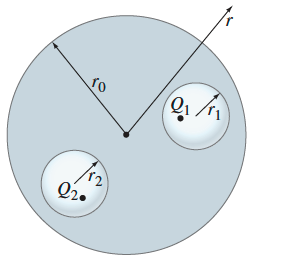
\includegraphics[width=0.30\textwidth]{./images/problems/lect04_sphere_with_2_cavities}\\
    \end{center}
  \end{blockexmplque}

\end{frame}

%
%
%

\begin{frame}{Worked example: Conducting sphere with cavities}

  Since the sphere is conducting, the electric field within that sphere
  will always be zero.\\
  \vspace{0.2cm}

  When charge $Q_1$ is brought in the first cavity, it creates an
  electric field within that cavity. Free charge carriers from the conducting
  sphere, with total charge of -$Q_1$, will distribute themselves on the
  surface of the cavity and shield the cavity charge, so that the electric field
  within the conducting sphere remains zero. The charge -$Q_1$ distrubuted
  on the surface of the cavity, will not be symetrically distributed.\\
  \vspace{0.2cm}

  Likewise, when charge $Q_2$ is brought in the second cacity,
  charge -$Q_2$ will be asymetrically distributed on the surface of the
  second cavity to shield $Q_2$ and ensure that the field is zero within the
  conductor.\\
  \vspace{0.2cm}

  Since the conducting sphere was not charged, the accumulation of charge
  -$Q_1$-$Q_2$ on the surface of the cavities, means that charge $Q_1$+$Q_2$
  will be accumulated on the outer surface of the sphere.\\

\end{frame}

%
%
%

\begin{frame}{Worked example: Conducting sphere with cavities}

  Since there is no electric field in the conductor, the influence of the
  inner charges doesn't extend to the outer surface, and the charge
  $Q_1$+$Q_2$ will be uniformly distributed on that surface.\\
  \vspace{0.1cm}

  The electric field outside the sphere can be found using
  Gauss's law:
   \begin{equation*}
     \oint_{S} \vec{E} \cdot d\vec{S} = \frac{Q_{encl}}{\epsilon_0}
   \end{equation*}
  If $S$ is a spherical surface with radius $r$ ($>r_0$),
  concentric with the conducting sphere, the symmetry of the problem
  suggests that:
  \begin{equation*}
    E 4\pi r^2 = \frac{Q_1 + Q_2}{\epsilon_0} \Rightarrow
    E = \frac{Q_1 + Q_2}{4\pi \epsilon_0 r^2}
  \end{equation*}
  This electric field is radial, so in vector form it can be written as:
  \begin{equation*}
    \vec{E} = \frac{Q_1 + Q_2}{4\pi \epsilon_0 r^2} \hat{r}
  \end{equation*}

  If $Q_1 + Q_2 > 0$ the electric field points outwards, whereas
  if $Q_1 + Q_2 < 0$ the electric field points inwards.

\end{frame}

} % Worked example

% ------------------------------------------------------------------------------

%
% Worked example : Water molecule
%

{
\problemslide

%
%
%

\begin{frame}{Worked example: Dipole moment of water molecule}

  \begin{blockexmplque}{Question}
     The dipole moment, considered as a vector, points from the negative to
     the positive charge. The water molecule, shown schematically below,
     has a dipole moment $\vec{p}$ which can be considered as the vector sum
     of the two dipole moments $\vec{p}_1$ and $\vec{p}_2$ as shown.
     The distance between each  H atom and O atom is about
     0.96 $\times$ 10$^{-10}$ m. The lines joining the centre of the O atom
     and each H atom make an angle of 104$^o$ as shown, and the net
     magnetic moment has been measured to be $p$ = 6.1 $\times$ 10$^{-30}$ C$\cdot$m.
    \begin{center}
      \includegraphics[width=0.33\textwidth]{./images/problems/lect04_water_dipole_2}\\
    \end{center}
  \end{blockexmplque}

\end{frame}

%
%
%

\begin{frame}{Worked example: Dipole moment of water molecule}

  \begin{blockexmplque}{Question}
    \begin{itemize}
      \item
      Determine the effective charge of each H atom.
      \item
      Determine the electric potential, far from the molecule,
      due to each dipole, $\vec{p}_1$ and $\vec{p}_2$,
      and show that
      \begin{equation*}
         V = \frac{1}{4\pi \epsilon_0} \frac{p cos\theta}{r^2}
      \end{equation*}
      where $p$ is the magnitude of the net dipole moment,
      $\vec{p}$ = $\vec{p}_1$ + $\vec{p}_2$,
      and $V$ is the total potential due to both $\vec{p}_1$ and $\vec{p}_2$.\\
      Take $V$ = 0 at infinity.\\
      Note that the potential of each dipole $\vec{p}_i$ ($i$=1,2) is given by:
      \begin{equation*}
         V = \frac{1}{4\pi \epsilon_0} \frac{\vec{p}_i \cdot \hat{r}}{r^2}
      \end{equation*}
    \end{itemize}
  \end{blockexmplque}

\end{frame}

%
%
%

\begin{frame}{Worked example: Dipole moment of water molecule}

  The two H-O pairs have equal electric dipole moment magnitudes:
  \begin{equation*}
    p_1 = p_2
  \end{equation*}
  given by:
  \begin{equation*}
    p_{1,2} = q d
  \end{equation*}
  Therefore, the total electric dipole moment:
  \begin{equation*}
    \vec{p} = \vec{p}_1 + \vec{p}_2
  \end{equation*}
  has a magnitude given by:
  \begin{equation*}
    p = p_1 cos(52^o) + p_2 cos(52^o) = 2 q d cos(52^o)
  \end{equation*}
  The above, yields the following expression for the effective charge $q$:
  \begin{equation*}
    q = \frac{p}{2 d cos(52^o)} \Rightarrow
  \end{equation*}

  \begin{equation*}
    q = \frac{6.1 \times 10^{-30} \; C \cdot m}{2 (0.96 times 10^{-10} \; m) cos(52^o)}
      = 5.2 \times 10^{-20} \; C
  \end{equation*}

\end{frame}

%
%
%

\begin{frame}{Worked example: Dipole moment of water molecule}

The potential $V$ of the water molecule can be written as:
  \begin{equation*}
    V = V_1 + V_2
  \end{equation*}

where $V_1$, $V_2$ is potential due to each H-O pair, given by:
  \begin{equation*}
    V_{1,2} = \frac{1}{4\pi \epsilon_0} \frac{\vec{p}_{1,2} \cdot \hat{r}}{r^2}
  \end{equation*}

Expanding the expressions for $V_1$, $V_2$, we find:
  \begin{equation*}
    V_1 = \frac{1}{4\pi \epsilon_0} \frac{\vec{p}_1 \cdot \hat{r}}{r^2}
        = \frac{1}{4\pi \epsilon_0} \frac{qd cos(52^o - \theta)}{r^2}
  \end{equation*}

  \begin{equation*}
    V_2 = \frac{1}{4\pi \epsilon_0} \frac{\vec{p}_2 \cdot \hat{r}}{r^2}
        = \frac{1}{4\pi \epsilon_0} \frac{qd cos(52^o + \theta)}{r^2}
  \end{equation*}

Therefore, $V$ can be written as:
  \begin{equation*}
    V = \frac{qd}{4\pi \epsilon_0 r^2}
       \Big( cos(52^o - \theta) + cos(52^o + \theta) \Big) \xRightarrow{p = 2 q d cos(52^o)}
  \end{equation*}

\end{frame}

%
%
%

\begin{frame}{Worked example: Dipole moment of water molecule}

  \begin{equation*}
    V = \frac{p}{8\pi \epsilon_0 cos(52^o) r^2}
       \Big( cos(52^o - \theta) + cos(52^o + \theta) \Big)
  \end{equation*}

Using the following trigonometric identity:
  \begin{equation*}
    cos(\alpha \pm \beta) = cos(\alpha) \; cos(\beta) \mp sin(\alpha) \; sin(\beta)
  \end{equation*}

we find:

  \begin{equation*}
    V = \frac{p}{8\pi \epsilon_0 \bcancel{cos(52^o)} r^2}
       \Big( \bcancel{cos(52^o)} cos(\theta) + \cancel{sin(52^o) sin(\theta)} +
             %\bcancel{cos(52^o)} cos(\theta) - \cancel{sin(52^o) sin(\theta)} \Big) \Rightarrow
  \end{equation*}
  \begin{equation*}
    %V = \frac{p}{8\pi \epsilon_0 \bcancel{cos(52^o)} r^2}
    %   \Big( \bcancel{cos(52^o)} cos(\theta) + \cancel{sin(52^o) sin(\theta)} +
             \bcancel{cos(52^o)} cos(\theta) - \cancel{sin(52^o) sin(\theta)} \Big) \Rightarrow
  \end{equation*}

  \begin{equation*}
    V = \frac{p cos(\theta)}{4\pi \epsilon_0 r^2}
  \end{equation*}

\end{frame}

} % Worked example

% ------------------------------------------------------------------------------
%
% Worked example :
%

{
\problemslide

%
%
%

\begin{frame}{Worked example: System of capacitors}

  \begin{blockexmplque}{Question}
    Three conducting plates, each of area $A$, are connected as shown below.
    \begin{center}
      \includegraphics[width=0.43\textwidth]{./images/problems/lect04_3_plane_capacitor}\\
    \end{center}
    \begin{itemize}
      \item Are the two capacitors thus formed connected in series or in parallel?
      \item Determine the net capacitance $C$ as a function of $d_1$, $d_2$, and $A$.
      \item The middle plate can be moved (changing the values of $d_1$, and $d_2$),
      to vary the capacitance. What are the minimum and the maximum values of the net capacitance?
    \end{itemize}
  \end{blockexmplque}

\end{frame}

%
%
%

\begin{frame}{Worked example: System of capacitors}

  The two capacitors are connected in parallel.\\
  \vspace{0.2cm}

  Let $C_1$, $C_2$ be the capacitances of the two parallel plane capacitors.
  They are given by:
  \begin{equation*}
    C_{1,2} = \epsilon_0 \frac{A}{d_{1,2}}
  \end{equation*}

  The total capacitance $C$ of the two capacitors connected in parallel is:
  \begin{equation*}
    C = C_1 + C_2
  \end{equation*}

  Substituting above the expression for $C_1$, $C_2$, we find:
  \begin{equation*}
    C = \epsilon_0 A \Big(\frac{1}{d_1} + \frac{1}{d_2}\Big)
      = \epsilon_0 A \frac{d_1 + d_2}{d_1 d_2}
  \end{equation*}

  As the middle plane moves, $d_1$ and $d_2$ change but
  $\ell = d_1 + d_2$ remains constant.
  Using $\ell$ and setting $d_1 = x$,
  the capacitance $C$ can be written as:
  \begin{equation*}
    C(x) = \epsilon_0 A \frac{\ell}{x (\ell-x)}
  \end{equation*}

\end{frame}

%
%
%

\begin{frame}{Worked example: System of capacitors}

  As $x \rightarrow 0$ and $x \rightarrow \ell$, $C = C_{max} \rightarrow \infty$.

  Between these maximum values at the extreme value of $x$, the capacitance
  reaches a minimum value which can be found by demanding that:
  \begin{equation*}
    \frac{dC(x)}{dx} = 0
  \end{equation*}

  Substituting the expression for $C$, the above becomes:
  \begin{equation*}
    \frac{d}{dx} \Big( \epsilon_0 A \frac{\ell}{x (\ell-x)} \Big) = 0 \Rightarrow
    \frac{d}{dx} \Big( \frac{1}{x (\ell-x)} \Big) = 0 \Rightarrow
    \frac{\ell - 2x}{(x(\ell-x))^2} = 0 \Rightarrow x = \frac{\ell}{2}
  \end{equation*}

  Therefore:
  \begin{equation*}
    C_{min} = C(x=\frac{\ell}{2}) =
      \epsilon_0 A \frac{\ell}{\frac{\ell}{2}(\ell-\frac{\ell}{2})} \Rightarrow
  \end{equation*}

  \begin{equation*}
    C_{min} = \frac{4 \epsilon_0 A}{\ell}
  \end{equation*}

\end{frame}


} % Worked example


% ------------------------------------------------------------------------------
% ------------------------------------------------------------------------------
